\documentclass[11pt,oneside,letterpaper]{article}

% graphicx package, useful for including eps and pdf graphics
\usepackage{graphicx}
\usepackage{grffile}
\usepackage{subfig}
%\DeclareGraphicsExtensions{.pdf,.png,.jpg}

% basic packages
\usepackage{color}
\usepackage{parskip}
\usepackage{float}
\usepackage{microtype}
\usepackage{url}
\urlstyle{same}

\usepackage[hidelinks]{hyperref}
\hypersetup{colorlinks=true,linkcolor=black,citecolor=black,urlcolor=black}

\usepackage{longtable}
\usepackage[]{algorithm2e}

% reference figures across documents
\usepackage{xr}
\externaldocument{mers-structure_supp}

% text layout
\usepackage{geometry}
\geometry{textwidth=15cm} % 15.25cm for single-space, 16.25cm for double-space
\geometry{textheight=22cm} % 22cm for single-space, 22.5cm for double-space

% helps to keep figures from being orphaned on a page by themselves
\renewcommand{\topfraction}{0.85}
\renewcommand{\textfraction}{0.1}

% bold the 'Figure #' in the caption and separate it with a period
% Captions will be left justified
\usepackage[labelfont=bf,labelsep=period,font=small]{caption}

% review layout with double-spacing
%\usepackage{setspace}
%\doublespacing
%\captionsetup{labelfont=bf,labelsep=period,font=doublespacing}

% cite package, to clean up citations in the main text. Do not remove.
%\usepackage{cite}
\usepackage{natbib}
%\renewcommand\citepleft{(}
%\renewcommand\citepright{)}
%\renewcommand\citepform[1]{\textsl{#1}}

\usepackage{amsmath}

\usepackage{lineno}
\linenumbers

% Remove brackets from numbering in list of References
%\renewcommand\refname{\large References}
%\makeatletter
%\renewcommand{\@biblabel}[1]{\quad#1.}
%\makeatother

\usepackage{authblk}
\renewcommand\Authands{ \& }
\renewcommand\Authfont{\normalsize \bf}
\renewcommand\Affilfont{\small \normalfont}
\makeatletter
\renewcommand\AB@affilsepx{, \protect\Affilfont}
\makeatother

% comments
\usepackage{ulem}
\definecolor{purple}{rgb}{0.459,0.109,0.538}
\def\tb#1#2{\sout{#1} \textcolor{purple}{#2}}
\def\tbc#1{\textcolor{purple}{[#1]}}
\def\gdc#1{\textcolor{blue}{[#1]}}
\def\lmc#1{\textcolor{green}{[#1]}}

% symbols
% \newcommand{\chiSq}{\chi^{2}_{df}} %LM: ancient DNA? =P %GD: quite :)
% \newcommand{\dtmrca}{\Delta_\mathrm{TMRCA}}
% \newcommand{\undtmrca}{\delta_\mathrm{TMRCA}}
% \newcommand{\dspr}{d_\mathrm{SPR}}

%%% TITLE %%%
\title{\vspace{1.0cm} \LARGE \bf MERS-CoV spillover at the camel-human interface}

\author[1]{Gytis Dudas}
\author[2]{Luiz Max Carvalho}
\author[2,3,4]{Andrew Rambaut}
\author[1]{Trevor Bedford}

\affil[1]{Vaccine and Infectious Disease Division, Fred Hutchinson Cancer Research Center, Seattle, WA, USA}
\affil[2]{Institute of Evolutionary Biology, University of Edinburgh, Edinburgh, UK}
\affil[3]{Fogarty International Center, National Institutes of Health, Bethesda, MD, USA}
\affil[4]{Centre for Immunology, Infection and Evolution at the University of Edinburgh, Edinburgh, UK}

% \date{\today}

\begin{document}
\maketitle

\begin{abstract}

Middle East respiratory syndrome coronavirus (MERS-CoV) is a zoonotic virus originating in camels that has been causing significant mortality and morbidity in humans in the Arabian Peninsula.
The epidemiology of the virus remains poorly understood, with hospital outbreaks, isolated cases with known exposure to camels and apparent community transmission occurring simultaneously.
While traditional and seroepidemiological studies have been employed extensively throughout the epidemic, viral sequence data have not been utilised to their full potential in understanding transmission patterns within the outbreak.
Here we use existing MERS-CoV sequence data to explore the phylodynamics of the virus in two of its known major hosts, humans and camels.
We employ structured coalescent models to show that long-term MERS-CoV evolution occurs exclusively in camels, whereas humans act as a transient, and ultimately terminal host.
By analysing the distribution of human outbreak cluster sizes and zoonotic introduction times we show that human outbreaks in the Arabian peninsula are driven by seasonally varying zoonotic transfer of viruses from camels.
Without heretofore unseen evolution of host tropism, MERS-CoV is unlikely to become endemic in humans.

\end{abstract}

\pagebreak

\section*{Introduction}
Middle East respiratory syndrome coronavirus (MERS-CoV), endemic in camels in the Arabian Peninsula, is the causative agent of zoonotic infections and limited outbreaks in humans.
The virus, first discovered in 2012 \citep{zaki_isolation_2012,boheemen_genomic_2012}, has caused more than 2000  infections and over 700 deaths, according to the World Health Organization (WHO) \citep{who_2017}.
Its epidemiology remains obscure, largely because infections are observed among the most severely affected individuals, such as older males with comorbidities \citep{assiri_2013,group_state_2013}.
While contact with camels is often reported, other patients do not recall contact with any livestock, suggesting an unobserved community contribution to the outbreak \citep{group_state_2013}.
Previous studies on MERS-CoV epidemiology have used serology to identify factors associated with MERS-CoV exposure in potential risk groups \citep{reusken_occupational_2015,reusken_2013}.
Such data have shown high seroprevalence in camels \citep{muller_2014,corman_antibodies_2014,chu_2014,reusken_2013,reusken_2014} and evidence of contact with MERS-CoV in workers with occupational exposure to camels \citep{reusken_occupational_2015,muller_presence_2015}.
Separately, epidemiological modelling approaches have been used to look at incidence reports through time, space and across hosts \citep{cauchemez_unraveling_2016}.


Although such traditional epidemiological approaches yield important clues about exposure patterns and potential for larger outbreaks, much inevitably remains opaque to such approaches due to difficulties in linking cases into transmission clusters in the absence of detailed information.
Genomic epidemiology, however, can fill this critical gap and has repeatedly shown the utility of viral sequence data in outbreak scenarios \citep{liu_h7n9_2013,gire_genomic_2014,grubaugh_multiple_2017}, where data are relatively cheap to produce.
These data can stand in for diagnostics and often yield a highly detailed picture of an epidemic when complete genome sequencing is performed consistently and appropriate metadata collected \citep{dudas_virus_2017}.
Sequence data can help discriminate between multiple and single source scenarios \citep{gire_genomic_2014}, which are fundamental to quantifying risk \citep{grubaugh_multiple_2017}.
Sequencing MERS-CoV has been performed as part of initial attempts to link human infections with the camel reservoir \citep{memish_human_2014}, nosocomial outbreak investigations \citep{assiri_hospital_2013} and routine surveillance \citep{park_acute_2015}.
A large portion of MERS-CoV sequences come from outbreaks within hospitals, where sequence data have been used to determine whether infections were isolated introductions or were part of a larger hospital-associated outbreak \citep{fagbo_molecular_2015}.
Similar studies on MERS-CoV have taken place at broader geographic scales, such as cities \citep{cotten_2013}.


It is widely accepted that recorded human MERS-CoV infections are a result of at least several introductions of the virus into humans \citep{cotten_2013} and that contact with camels is a major risk factor for developing MERS, per WHO guidelines \citep{who_2016_MERS}.
Previous studies attempting to quantify the actual number of spillover infections have either relied on traditional epidemiological approaches \citep{cauchemez_unraveling_2016} or employed methods agnostic to signals of population structure within sequence data \citep{zhang_evolutionary_2016}.
Here we use a dataset of 274 MERS-CoV genomes to investigate transmission patterns of the virus between humans and camels.

Here, we use an explicit model of metapopulation structure and migration between discrete subpopulations, referred to here as demes \citep{vaughan_efficient_2014}, derived from the structured coalescent \citep{notohara_structured_coalescent_1990}.
Unlike approaches that model host species as a discrete phylogenetic trait of the virus using continuous-time Markov processes (or simpler, parsimony based, approaches) \citep{faria_simultaneously_2013,lycett_h5n8_2016}, population structure models explicitly incorporate distinct sampling patterns, population dynamics within demes and migration between demes.
By estimating independent coalescence rates for MERS-CoV in humans and camels, as well as migration patterns between the two demes, we show that long-term viral evolution of MERS-CoV occurs exclusively in camels.
Our results suggest that spillover events into humans are seasonal and might be associated with the calving season in camels.
Once human MERS-CoV infections are established, however, we find that MERS-CoV is poor at transmitting between humans.
Using Monte Carlo simulations we show that $R_{0}$ for MERS-CoV circulating in humans is much lower than the epidemic threshold of 1.0 and that correspondingly the virus has been introduced into humans hundreds of times.

\section*{Results}

\subsection*{MERS-CoV is predominantly a camel virus}

The structured coalescent approach we employ (see Methods) identifies camels as a reservoir host where most of MERS-CoV evolution takes place (Figure \ref{mcc}), while human MERS outbreaks are transient and terminal with respect to long-term evolution of the virus (Figure~\ref{exploded}).
Across 174 MERS-CoV genomes collected from humans, we estimate a median of 56 separate camel-to-human cross-species transmissions (95\% highest posterior density (HPD): 48--63).
While we estimate a median of 3 (95\% HPD: 0--12) human-to-camel migrations, the 95\% HPD interval includes zero and we find that no such migrations are found in the maximum clade credibility tree (Figure~\ref{mcc}).
Correspondingly, we observe substantially higher camel-to-human migration rate estimates than human-to-camel migration rate estimates (Figure~\ref{prior}).
This inference derives from the tree structure wherein human viruses appear as clusters of highly related sequences nested within the diversity seen in camel viruses, which themselves show signicantly higher diversity and less clustering.
This manifests as different rates of coalescence with camel viruses showing a scaled effective population size $N_e \tau$ of 3.49 years (95\% HPD: 2.71--4.38) and human viruses showing a scaled effective population of 0.24 years (95\% HPD: 0.14--0.34).

We believe that the small number of inferred human-to-camel migrations are induced by the migration rate prior, while some are derived from phylogenetic proximity of human sequences to the apparent ``backbone'' of the phylogenetic tree.
This is most apparent in lineages in early-mid 2013 that lead up to sequences comprising the MERS-CoV clade dominant in 2015, where owing to poor sampling of MERS-CoV genetic diversity from camels the model cannot completely dismiss humans as a potential alternative host.
The first sequences of MERS-CoV from camels do not appear in our data until November 2013.
Our finding of negligible human-to-camel transmission is robust to choice of prior (Figure~\ref{prior}).

The repeated and asymmetric introductions of short-lived clusters of MERS-CoV sequences from camels into humans leads us to conclude that MERS-CoV epidemiology in humans is dominated by zoonotic transmission (Figure~\ref{mcc} and~\ref{exploded}).
We observe dense terminal clusters of MERS-CoV circulating in humans that are of no subsequent relevance to the evolution of the virus.
These clusters of presumed human-to-human transmission are then embedded within extensive diversity of MERS-CoV lineages inferred to be circulating in camels, a classic pattern of source-sink dynamics.
Our analyses recover these results despite sequence data heavily skewed towards non-uniformly sampled human cases and are robust to choice of prior.
This suggests that instances of human infection with MERS-CoV are more common than currently thought, with exceedingly short transmission chains mostly limited to primary cases that might be mild and ultimately not detected by surveillance or sequencing.

\begin{figure}[h]
 \centering
	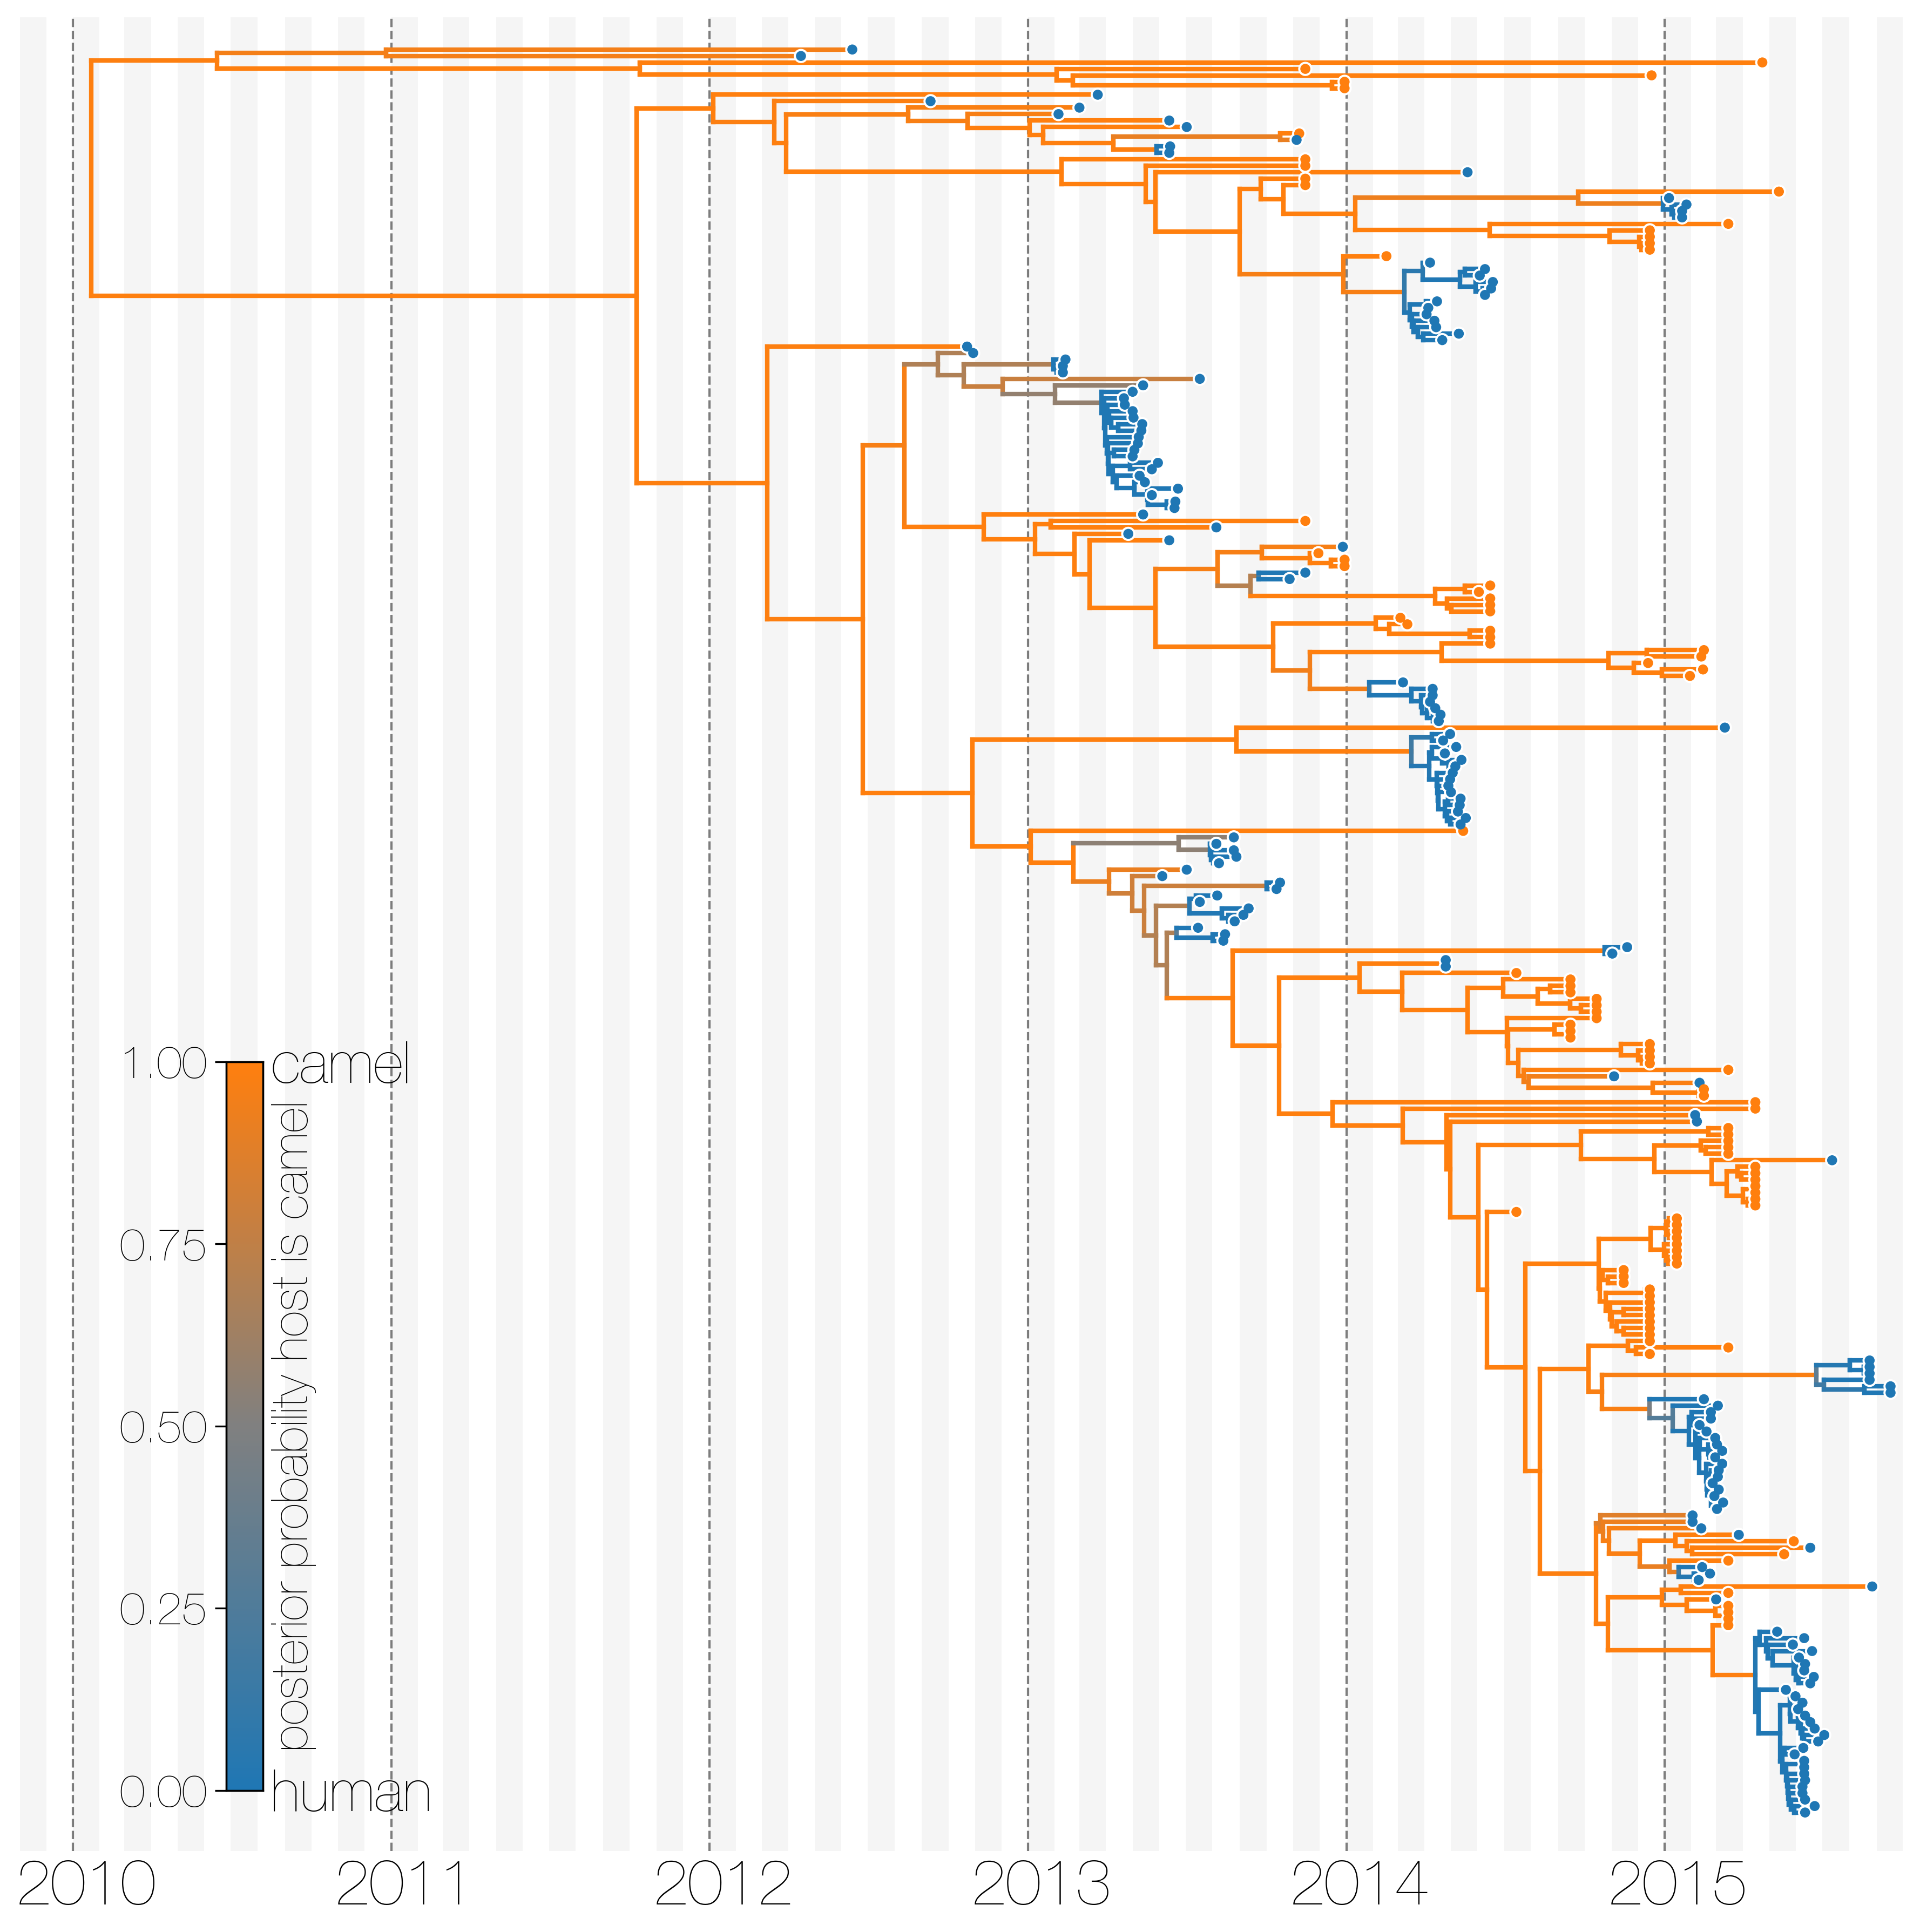
\includegraphics[width=0.75\textwidth]{figures/mers_mcc.png}
	\caption{\textbf{Typed maximum clade credibility tree of MERS-CoV genomes from 174 human viruses and 100 camel viruses.}
	Maximum clade credibility (MCC) tree showing inferred ancestral hosts for MERS-CoV recovered with the structured coalescent.
	The vast majority of MERS-CoV evolution is inferred to occur in camels (orange) with human outbreaks (blue) representing evolutionary dead-ends for the virus.
  Confidence in host assignment is depicted as a colour gradient, with increased uncertainty in host assignment (posterior probabilities close to 0.5) shown as grey.
	While large clusters of human cases are apparent in the tree, significant contributions to human outbreaks are made by singleton sequences, likely representing recent cross-species transmissions that were caught early.
	}
	\label{mcc}
\end{figure}

\subsection*{MERS-CoV shows seasonal introductions}
We use the posterior distribution of MERS-CoV introduction events from camels to humans (Figure \ref{mcc}) to model seasonal variation in zoonotic transfer of viruses.
We identify four months (April, May, June, July) when the odds of MERS-CoV introductions are increased (Figure \ref{seasonality}) and four when the odds are decreased (August, September, November, December).
Camel calving is reported to occur from October to February \citep{almutairi_non-genetic_2010}, with rapidly declining maternal antibody levels in calves within the first weeks after birth \citep{wernery_camelid_2001}.
It is possible that MERS-CoV sweeps through each new camel generation once critical mass of susceptibles is reached \citep{martinez_seasonality_2014}, leading to a sharp rise in prevalence of the virus in camels and resulting in increased force of infection into the human population.
Strong influx of susceptibles and subsequent sweeping outbreaks in camels may explain evidence of widespread exposure to MERS-CoV in camels from seroepidemiology \citep{muller_2014,corman_antibodies_2014,chu_2014,reusken_2013,reusken_2014}.

Although we find evidence of seasonality in zoonotic spillover timing, no such relationship exists for sizes of human sequence clusters \tbc{reference a figure}.
This is entirely expected, since little seasonality in human behaviour that could facilitate MERS-CoV transmission is expected following an introduction.
Similarly, we do not observe any trend in human sequence cluster sizes over time (Figure \ref{seasonality}B, Spearman $\rho = 0.06$, $p=0.68$), suggesting that MERS-CoV outbreaks in humans are neither growing nor shrinking in size.
This is not surprising either, since MERS-CoV is a camel virus that has to date, experienced little-to-no selective pressure to improve transmissibility between humans.

\begin{figure}[h]
\centering
	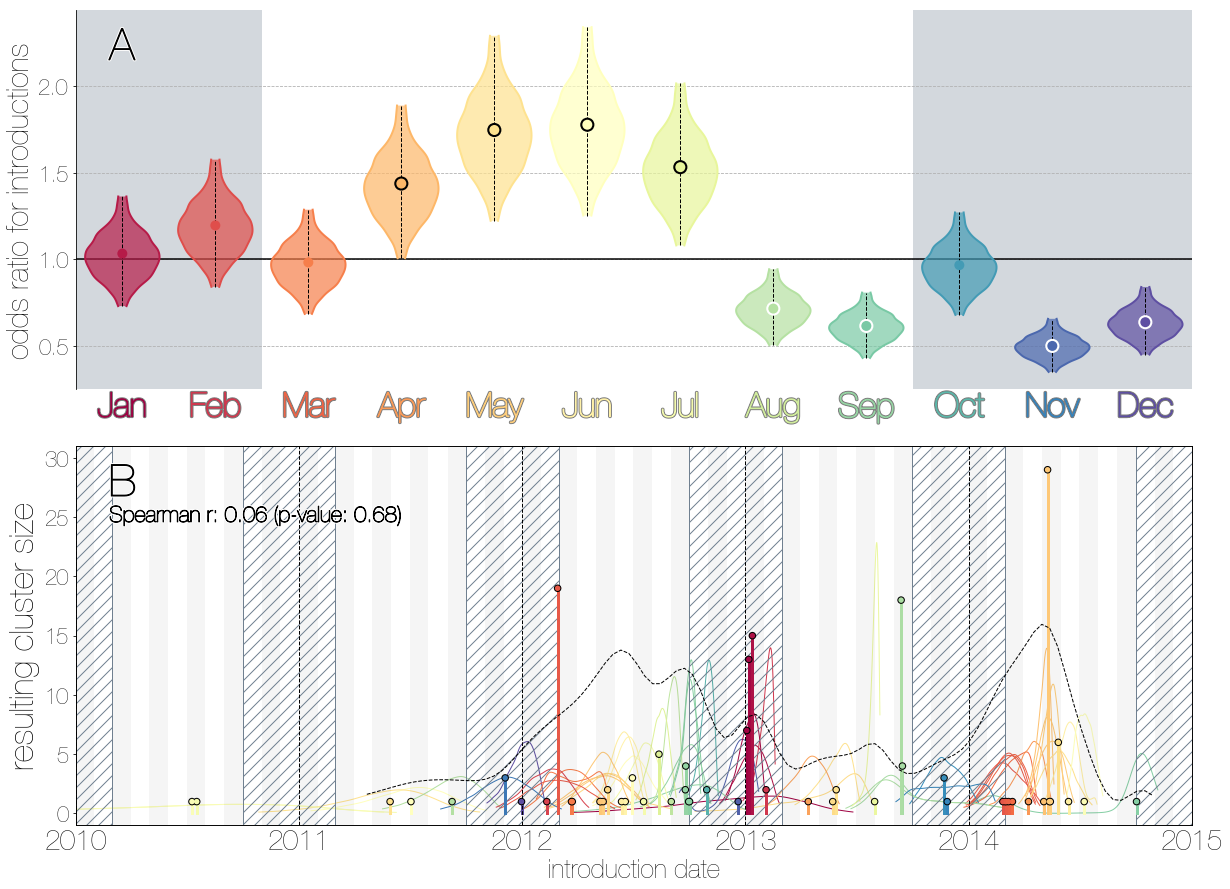
\includegraphics[width=0.75\textwidth]{figures/mers_seasonality.png}
	\caption{\textbf{Seasonality of MERS-CoV introduction events.}
A) Posterior density estimates partitioned by month showing the 95\% highest posterior density interval for relative odds ratios of MERS-CoV introductions into humans.
Posterior means are indicated with circles.
Evidence for increased or decreased risk (95\% HPD excludes 1.0) for introductions are indicated by black or white circles, respectively.
Hatched area spanning October to February indicates the camel calving season.
B) Sequence cluster sizes and inferred dates of introduction events.
Each introduction event is shown as a vertical line positioned based on the median introduction time, as recovered by structured coalescent analyses and coloured by time of year with height indicating number of descendant sequences recovered from human cases.
95\% highest posterior density intervals for introductions of MERS-CoV into humans are indicated with coloured lines, coloured by median estimated introduction time.
The black dotted line indicates the joint probability density for introductions.
We find little correlation between date and size of introduction (Spearman $\rho = 0.06$, $p=0.68$).
	}
	\label{seasonality}
\end{figure}

\subsection*{MERS-CoV is poorly suited for human transmission}

Structured coalescent approaches clearly show humans to be a terminal host for MERS-CoV, implying poor transmissibility.
However, we wanted to translate this observation into an estimate of the basic reproductive number, $R_{0}$, which is more familiar to epidemiologists and provides insight into epidemic behavior.
The parameter $R_{0}$ determines expected number of secondary cases in a single infections as well as the distribution of total cases that result from a single introduction event into the human population (Equation~\ref{clusterLikelihood}, Methods).
We estimate $R_{0}$ along with other relevant parameters via Monte Carlo simulation in two steps.
First, we simulate case counts across multiple outbreaks totaling 2000 cases using Equation \ref{clusterLikelihood} and then we subsample from each case cluster to simulate sequencing of a fraction of cases.
Sequencing simulations take place at different levels of bias, wherein bias enriches sequencing of larger case clusters.
This is a particularly pressing issue, since \textit{a priori} we expect large hospital outbreaks of MERS to be overrepresented in sequence data, whereas sequences from primary cases will be sampled exceedingly rarely.
We record the mean, median and standard deviation of sequence cluster sizes in each simulation (left-hand panels in Figure \ref{mers_epi}) and extract the subset of Monte Carlo simulations in which these summary statistics fall within the 95\% highest posterior density observed in the empirical MERS-CoV data from structured coalescent analyses.
We record $R_{0}$ values, as well as the number of case clusters (equivalent to number of zoonotic introductions), for these empirically matched simulations.
A schematic of this Monte Carlo produre is shown in Figure \ref{mc_method}.
Generally, higher $R_0$ results in fewer larger transmission clusters, while lower $R_0$ results in many smaller transmission clusters (Figure \ref{mers_epi}).

We find that observed phylogenetic patterns of sequence clustering strongly support $R_{0}$ below 1.0 (middle panels in Figure \ref{mers_epi}).
For increasing levels of bias mean $R_{0}$ values observed in matching simulations are 0.844, 0.730, and 0.683, respectively.
While the 95\% percentiles for $R_{0}$ values are close to 1.0 (0.720--0.995) for the unbiased sequencing simulation (\textit{i.e.}\ uniform sequencing efforts, in which every case is equally likely to be sequenced), we also note that increasing levels of bias are considerably more to likely to generate MERS-CoV-like sequence clusters (Figure \ref{mers_epi}).
Under unbiased sequencing only 0.6\% of simulations fit our phylogenetic observations, while 2.7\% and 2.7\% of simulations fit for bias levels of 2.0 and 3.0, respectively.
Correspondingly, we estimate 10\% support for a model with bias level 1.0, 45\% support for a model with bias level 2.0, and 45\% support for a model with bias level 3.0.
Model averaging would suggest plausible $R_0$ values between 0.57 and 0.91.

Lower values for $R_{0}$ in turn suggest relatively large numbers of zoonotic transfers of viruses into humans (right-hand panels in Figure \ref{mers_epi}).
The median number of cross-species introductions observed in simulations matching empirical data without bias are 339 (95\% percentiles 255--431).
These numbers jump up to 558 (95\% percentiles 424--720) for bias = 2 and 650 (95\% percentiles 481--850) for bias = 3 simulations, which as mentioned previously match considerably better to MERS phylogenetic data.
Model averaging would suggest plausible numbers of introductions between 299 and 818.
Our results suggest a large number of unobserved MERS primary cases.
Given this, we also performed simulations where the total number of cases is doubled to 4000 to explore the impact of dramatic underestimation of MERS cases.
In these analyses $R_{0}$ values tend to decrease even further as numbers of introductions go up, although very few simulations match currently observed MERS-CoV sequence data (Figure \ref{extra_cases}).

Overall, our analyses indicate that MERS-CoV is poorly suited for human-to-human transmission, with an estimated $R_{0}<0.91$ and sequence sampling likely to be biased towards large hospital outbreaks.
Given these findings, and the fact that large outbreaks of MERS occurred in hospitals, the combination of frequent spillover of MERS-CoV into humans and occasional outbreak amplification via poor hygiene practices \citep{assiri_hospital_2013,chen_comparative_2017} appear sufficient to explain observed epidemiological patterns of MERS-CoV.

\begin{figure}[h]
\centering
	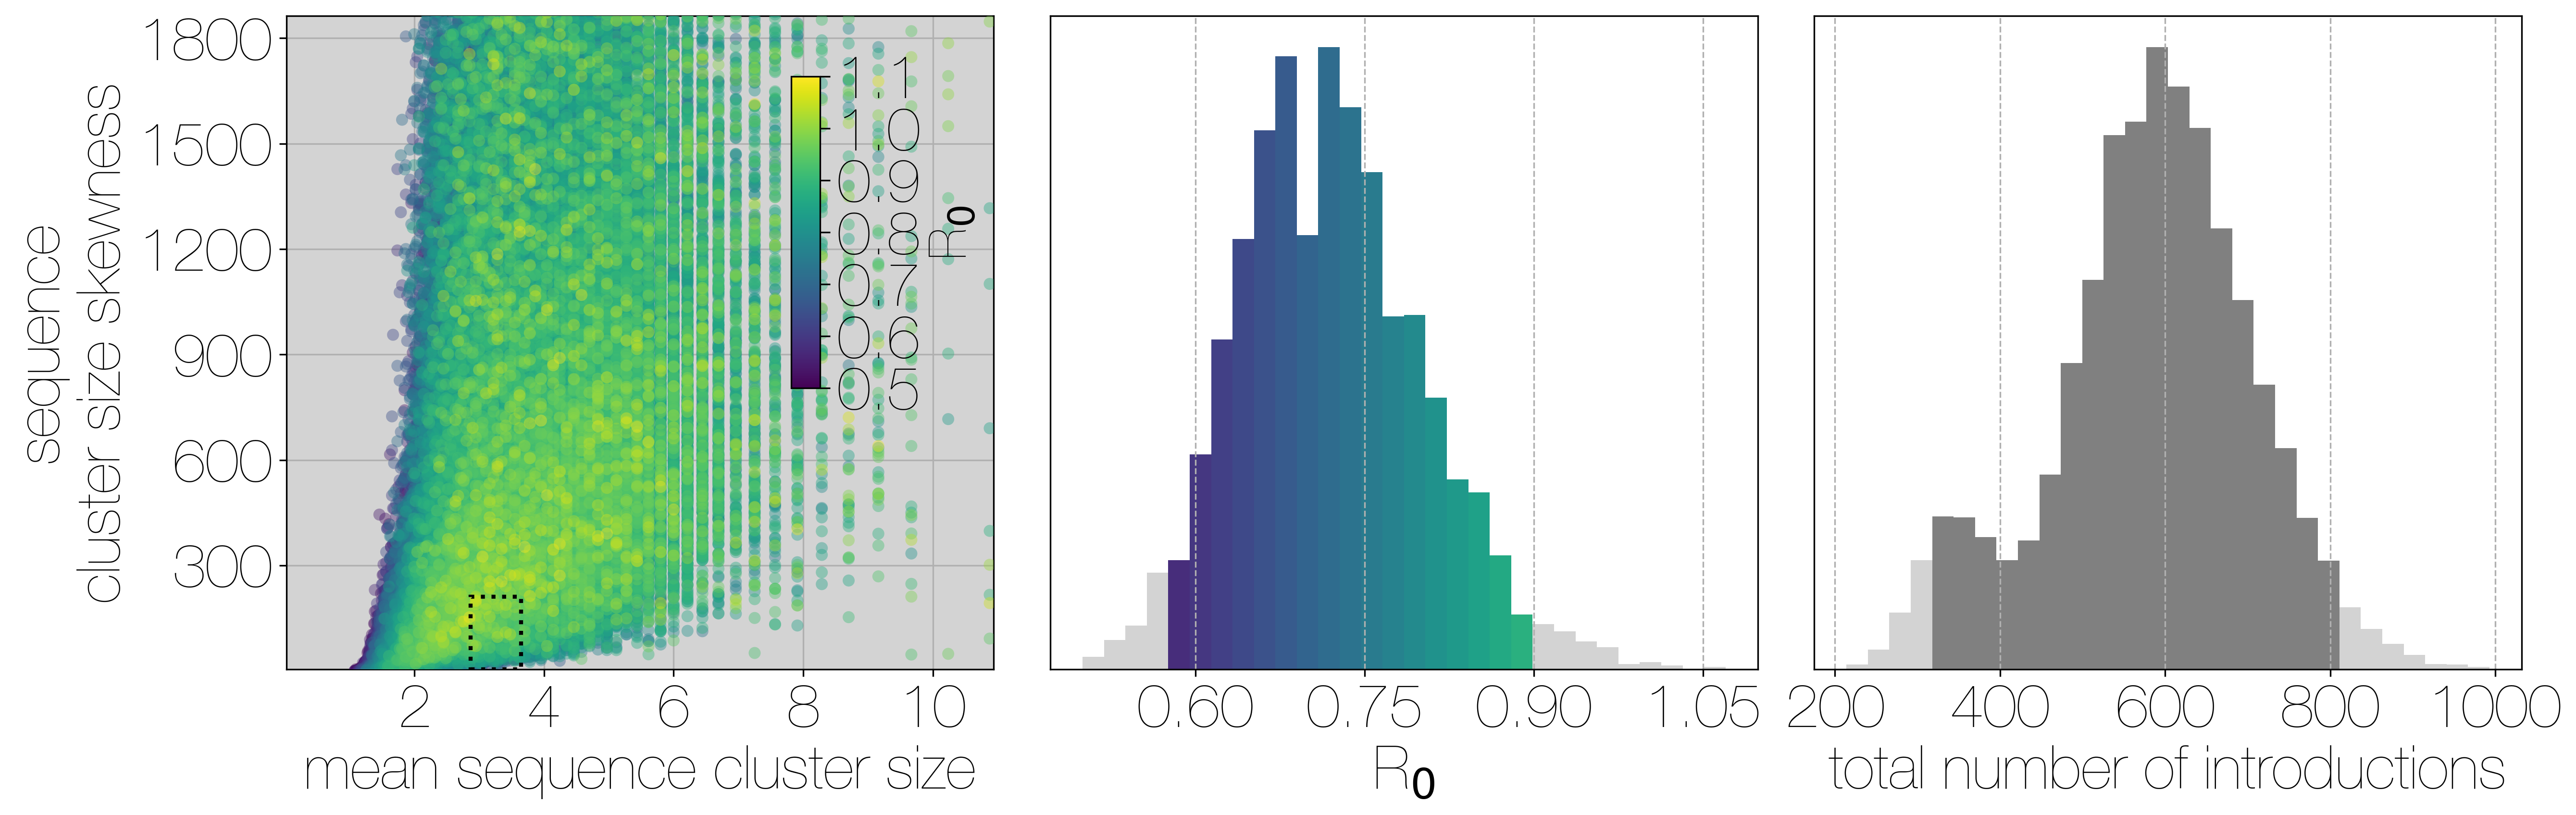
\includegraphics[width=0.75\textwidth]{figures/mers_epi.png}
	\caption{\textbf{Monte Carlo simulations of human transmission clusters.}
Each row corresponds to a different bias value used to concentrate the subsampling of sequences from cases, and goes from 1 (no bias) to 2, and 3 (increasing levels of bias which make large case clusters to be more likely to be sequenced).
Leftmost scatter plots show results of individual Monte Carlo simulations, coloured by the $R_{0}$ value used for the simulation.
The dotted rectangle identifies the 95\% highest posterior density bounds for sequence cluster size mean and standard deviation observed for empirical MERS-CoV data.
The distribution of $R_{0}$ values found within the dotted rectangle is shown in the middle, on the same $y$-axis across all levels of bias.
Bins falling inside the 95\% percentiles are coloured by $R_{0}$, as in the leftmost scatter plot.
The distribution of total number of introductions associated with simulations matching MERS-CoV sequence clusters is shown in the plots on the right, on the same $y$-axis across all levels of bias.
Darker shade of grey indicates bins falling within the 95\% percentiles.
These Monte Carlo simulations indicate $R_{0}$ for MERS-CoV is likely to be below 1.0, with biased sequencing and numbers of zoonotic transmissions numbering in the hundreds.
	}
	\label{mers_epi}
\end{figure}

\subsection*{Recombination shapes MERS-CoV diversity}
Recombination has been shown to occur in all genera of coronaviruses, including MERS-CoV \citep{lai_1985,makino_1986,keck_1988,kottier_1995,herrewegh_1998}. %\tbc{needs citations}.
In order to explore the role of recombination in shaping MERS-CoV genetic diversity we used two recombination detection approaches across partitions of taxa corresponding to inferred MERS-CoV clades.
Both methods rely on sampling parental and recombinant alleles within the alignment, although each quantifies different signals of recombination.
One hallmark of recombination is the ability to carry alleles derived via mutation from one lineage to another, which appear as repeated mutations taking place in the recipient lineage, somewhere else in the tree.
The PHI (pairwise homoplasy index) test quantifies the appearance of these excessive repeat mutations (homoplasies) within an alignment \citep{bruen_simple_2006}.
Another hallmark of recombination is spatial clustering of alleles along the genome, due to how template switching, the primary mechanism of recombination in RNA viruses, occurs.
3Seq relies on the spatial structure of nucleotide similarities between sequence triplets -- two potential parent-donors and one candidate offspring-recipient sequences \citep{boni_exact_2007}.

Both tests can give spurious results in cases of extreme rate heterogeneity and sampling over time \citep{dudas_mers-cov_2016}, but both tests have not been reported to fail simultaneously.
PHI and 3Seq methods consistently identify most of the apparent `backbone' of the MERS-CoV phylogeny as encompassing sequences with evidence of recombination (Figure \ref{recombination_tree}).
Neither method can identify where in the tree recombination occurred, but each full asterisk in Figure \ref{recombination_tree} should be interpreted as the minimum partition of data that still captures both donor and recipient alleles involved in a recombination event.
This suggests a non-negligible contribution of recombination in shaping existing MERS-CoV diversity.
As done previously \citep{dudas_mers-cov_2016}, we show large numbers of homoplasies in MERS-CoV data (Figure \ref{incompatibilities}) with some evidence of spatial clustering of such alleles.
% Homoplasies are present in multiple strains at a time, indicating recombination events that have been successful.
Although the evolutionary centrality of camel viruses (Figure \ref{mcc}) may be sufficient to argue that camels are the host where MERS-CoV recombines, incidence of MERS-CoV is known to be much higher in camels \citep{muller_2014,corman_antibodies_2014,chu_2014,reusken_2014,ali_systematic_2017}.
This provides ideal conditions for co-infection with distinct genotypes, which is a pre-requisite for detectable RNA virus recombination to occur.

%%% AR - this paragraph is a bit of a mess. Suggests we can't trust most of the analysis above. If we can't believe the camel tree why do we trust a structured coalescent model?
Conversely, our results strongly suggest that co-infection of humans with distinct lineages of MERS-CoV should be exceedingly rare.
We find little evidence that recombination will interfere with the inference of human outbreak clusters (Figure \ref{recombinant_features}A).
\tbc{Summarize Figure \ref{recombinant_features}A with something like: ``We find that 95\% of human viruses fall within the same introduction event in genomic fragment 1 and in genomic fragment 2.''}
And while we observe evidence of distinct phylogenetic trees from different parts of the MERS-CoV genome (Figure \ref{recombinant_features}B), human clades are minimally affected and large portions of the posterior probability density in both parts of the genome are concentrated in shared clades (Figure \ref{flower}).
Critically, we observe the same source-sink dynamics between camel and human populations in trees constructed from separate genomic fragments as were observed in the original full genome tree (Figures \ref{mcc}, \ref{recombinant_features}B).
Observed departures from strictly clonal evolution suggest that while recombination is an issue for inferring MERS-CoV phylogenies, its effect on the human side of MERS outbreaks is minimal, as expected.
MERS-CoV evolution on the reservoir side, though complicated by recombination, is nonetheless still amenable to phylogenetic methods, in part through limited diversity of the virus in camels (see next section).
In humans MERS-CoV evolution should be far easier to track as the only detectable and problematic recombinants are more likely to arise within the transmission chain, than through human co-infection with distinct MERS-CoV lineages.


% \begin{figure}[h]
%  \centering
% 	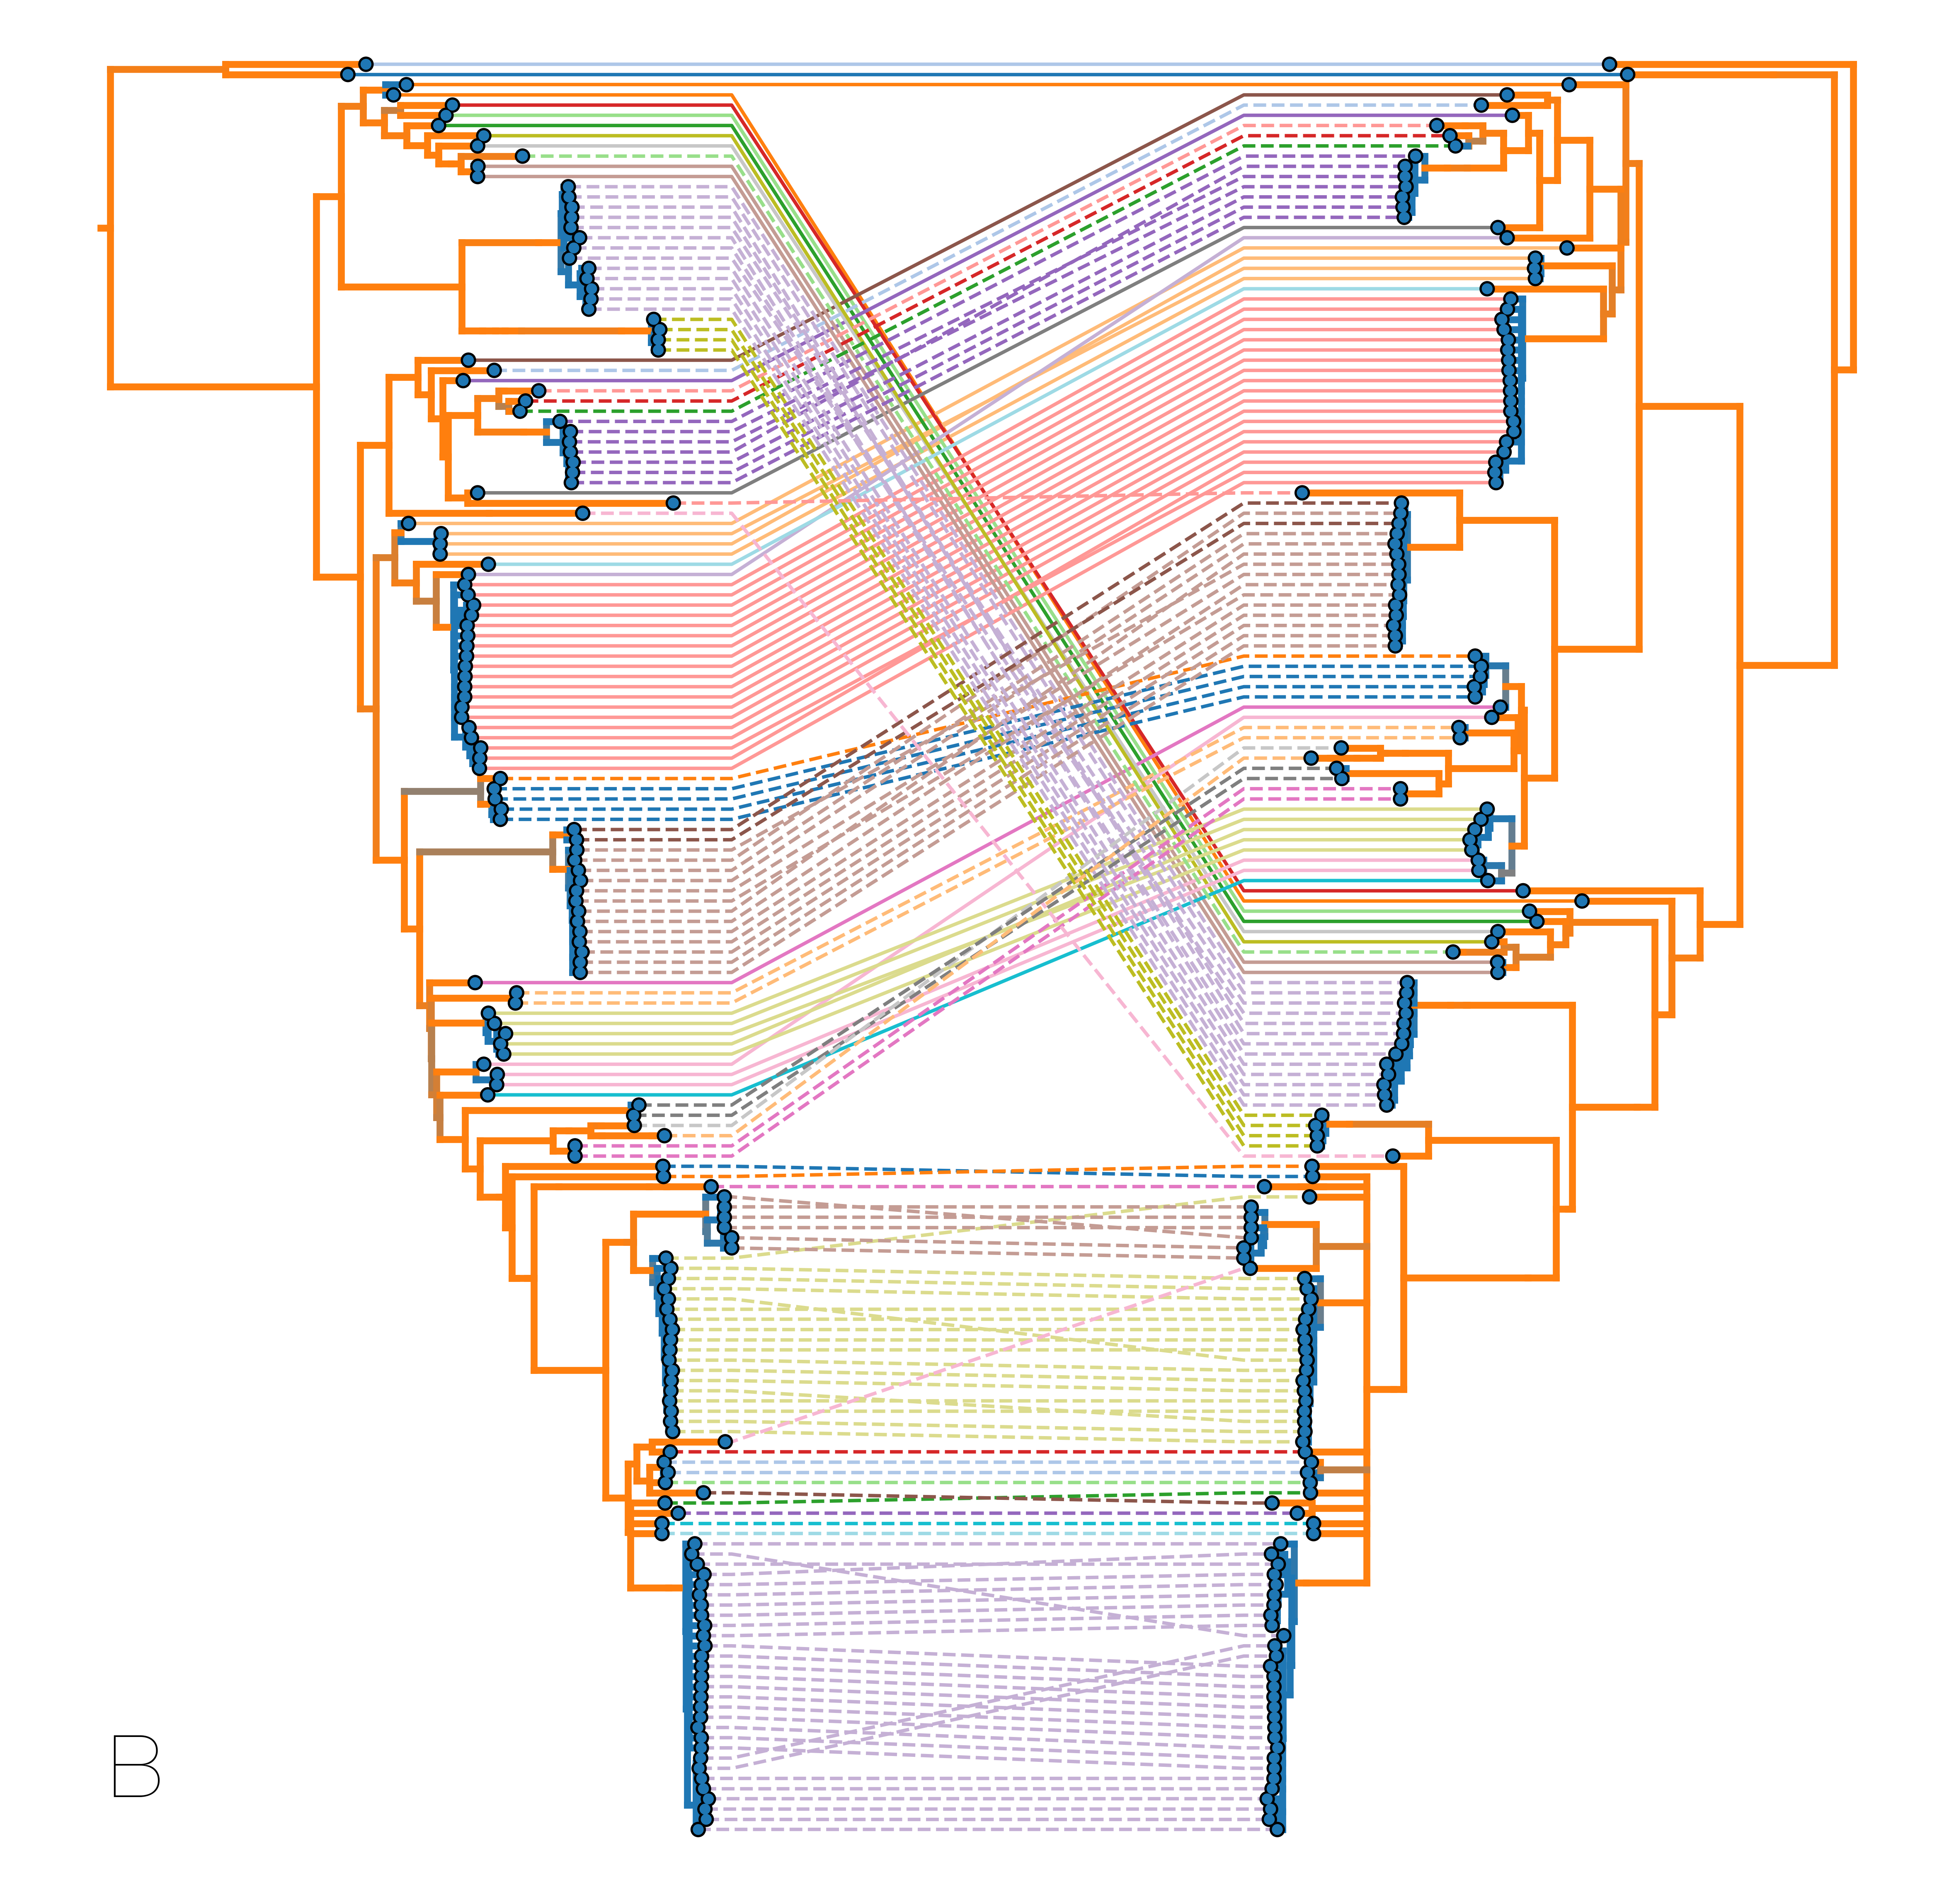
\includegraphics[width=0.65\textwidth]{figures/mers_chain.png}
%   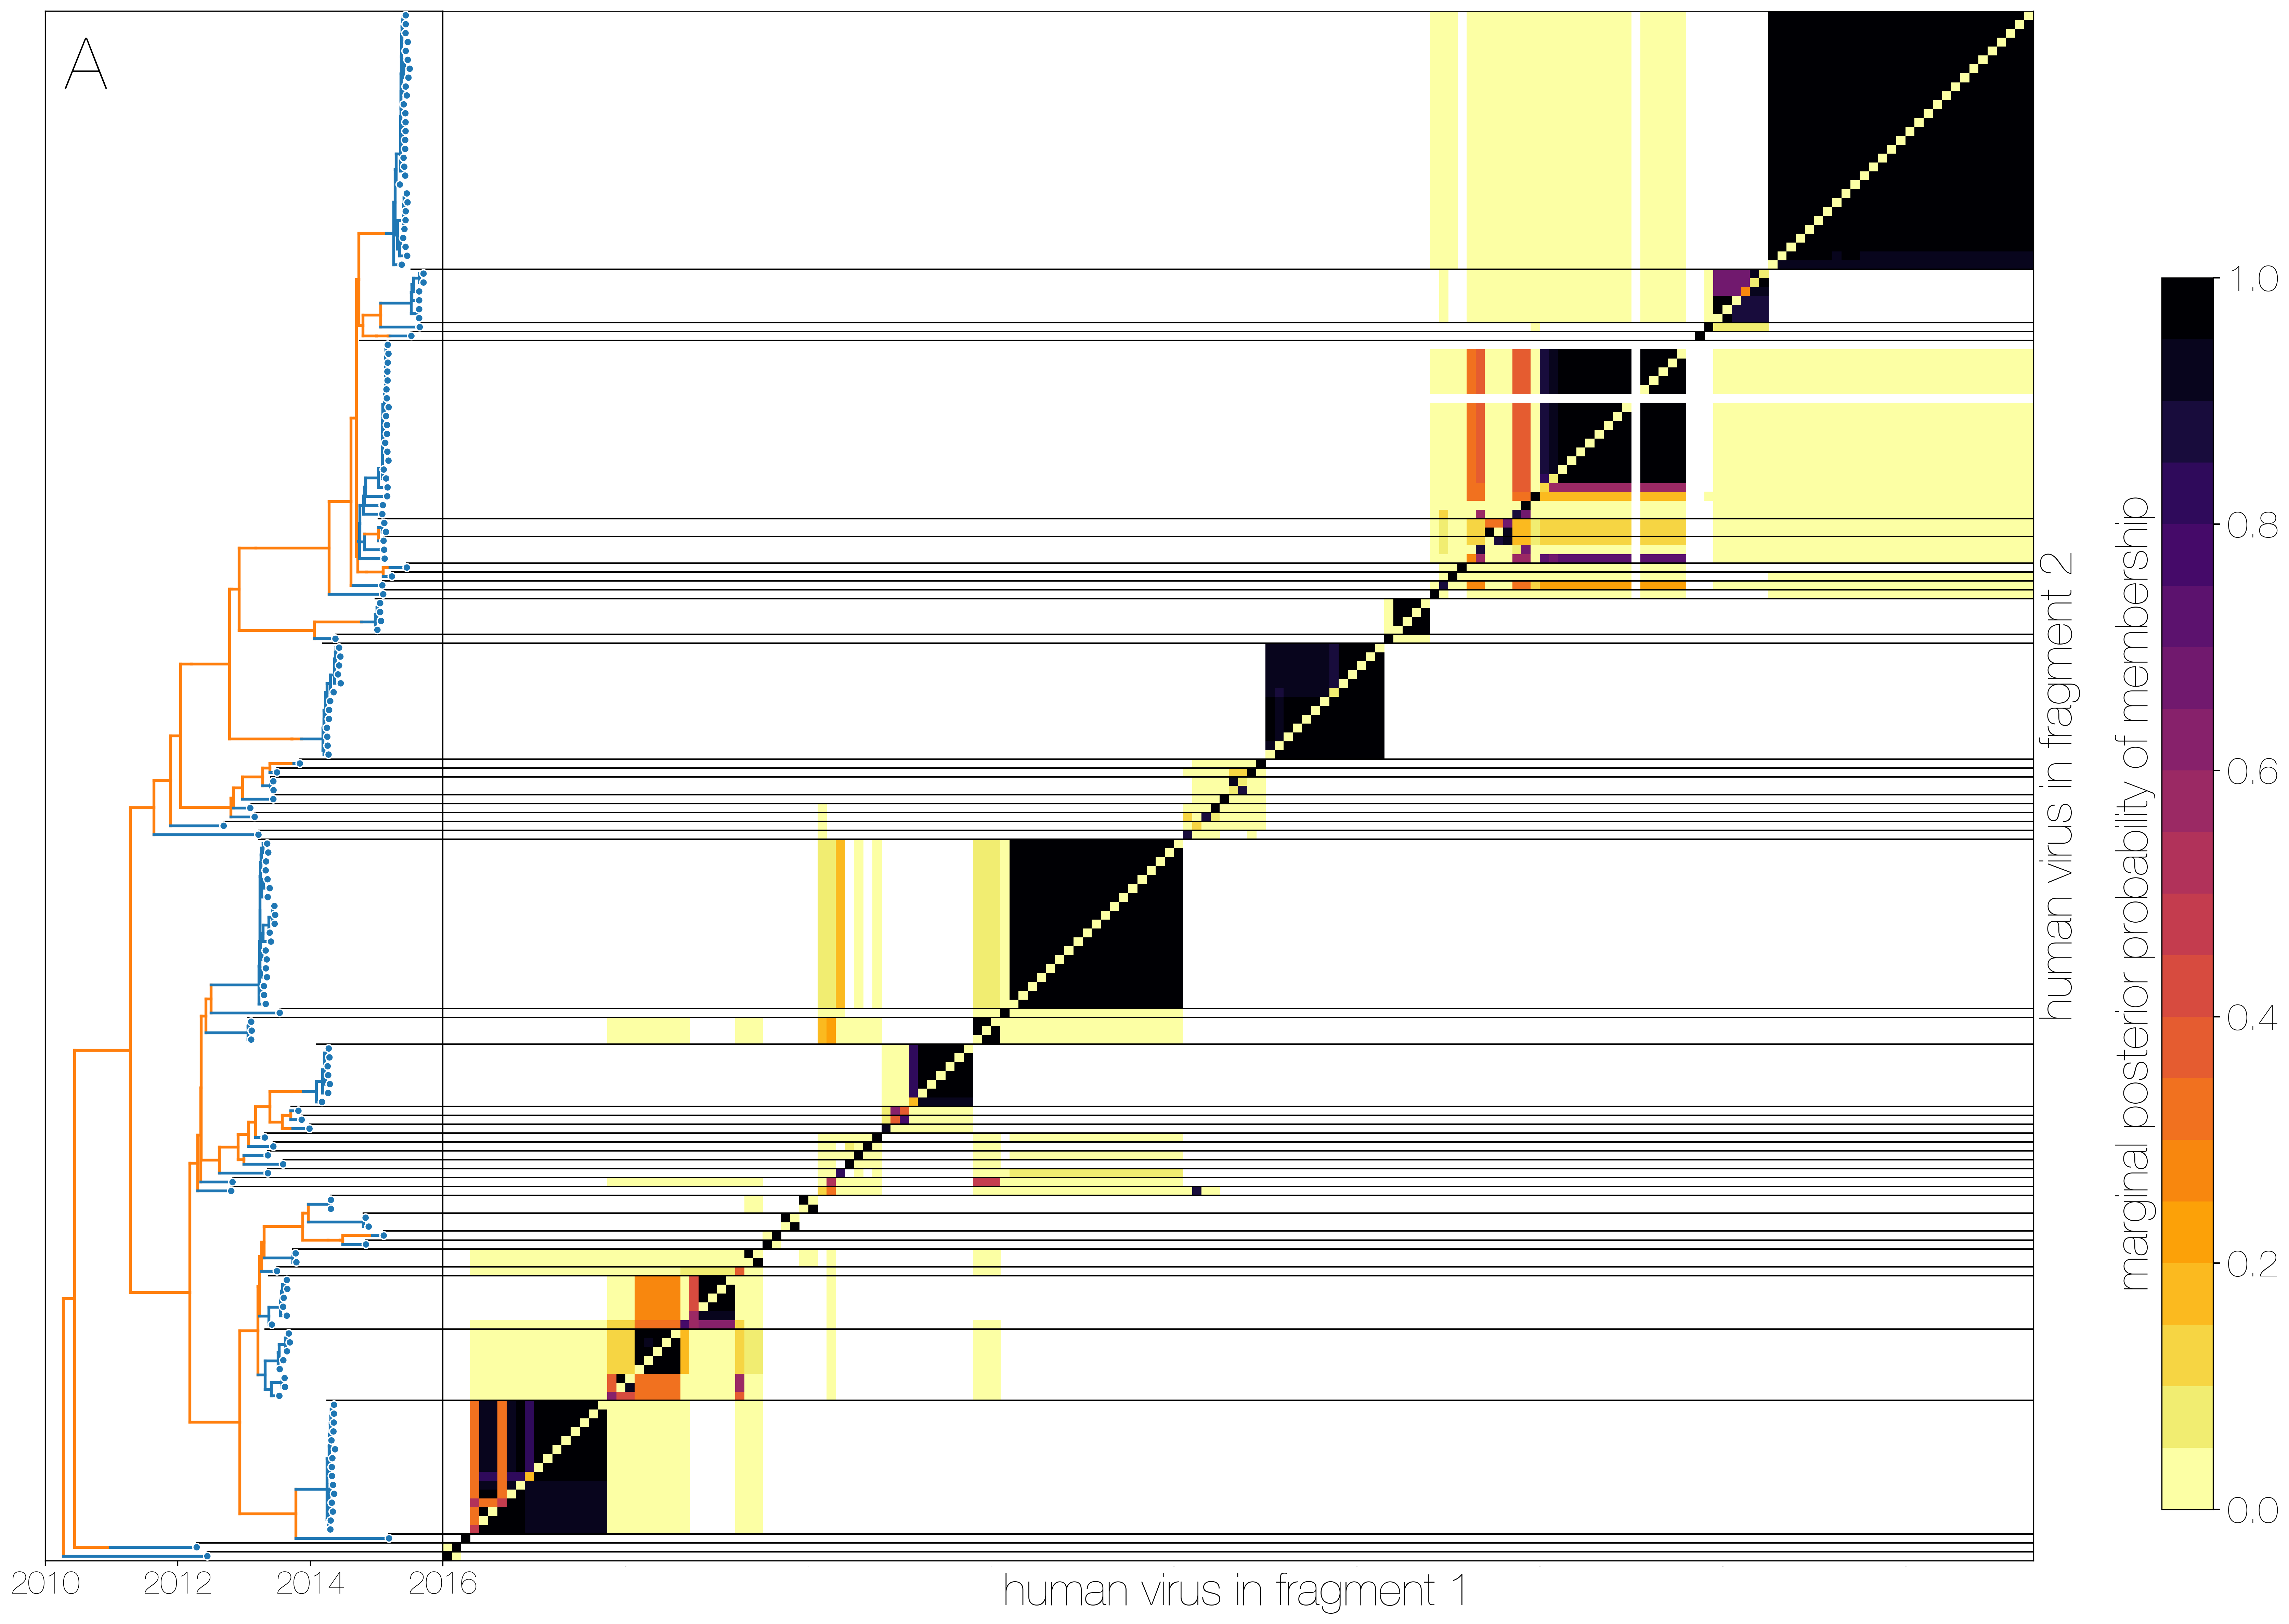
\includegraphics[width=0.65\textwidth]{figures/mers_fragments.png}
% 	\caption{\textbf{Tangled chain of MERS-CoV genome and its parts.}
% 	Tangled chain of the full genome (a), all nucleotides up to position 21000 (b) and all nucleotides past position 21000 (c) of MERS-CoV.
% 	The same taxa, if available in neighbouring trees, are connected via coloured lines (human sequences in blue, camel sequences in red).
% 	Tree branches are coloured by inferred ancestral host state (human in grey, camel in black).
% 	While some of apparent incongruities are caused by having less data in some of the fragments, inconsistencies between topologies occur across internal branches inferred to be in the camel host.
% 	Human clusters in grey change phylogenetic positions between the trees wholesale, with minor incongruences within clusters.
% 	This is evidence for recombinant viruses generated in the reservoir entering human populations.
% 	Coding sequences in the MERS-CoV genome are indicated with arrows at the bottom of the plot with position 21000 indicated by the black line.}
% 	\label{mers_chain}
% \end{figure}

% \begin{figure}[h]
% \centering
%
% 	\caption{\textbf{Pairwise co-occurence matrix for human clusters.}
% Heatmap shows the posterior probability that a pair of tips from trees of genomic fragments fall within the same clade - tips from fragment 1 are on the x axis, tips from fragment 2 are on the y axis.
% Tips are ordered by their appearance in tree of genome fragment 2 (positions from nucleotide 21000 onwards) reduced to just the human tips and coloured by inferred host (blue for human, orange for camel) on the left.
% Human clusters are largely well-supported as monophyletic and consistent across trees of both genomic fragments.
% 	}
% 	\label{coocurrence}
% \end{figure}
\begin{figure}%
    \centering
    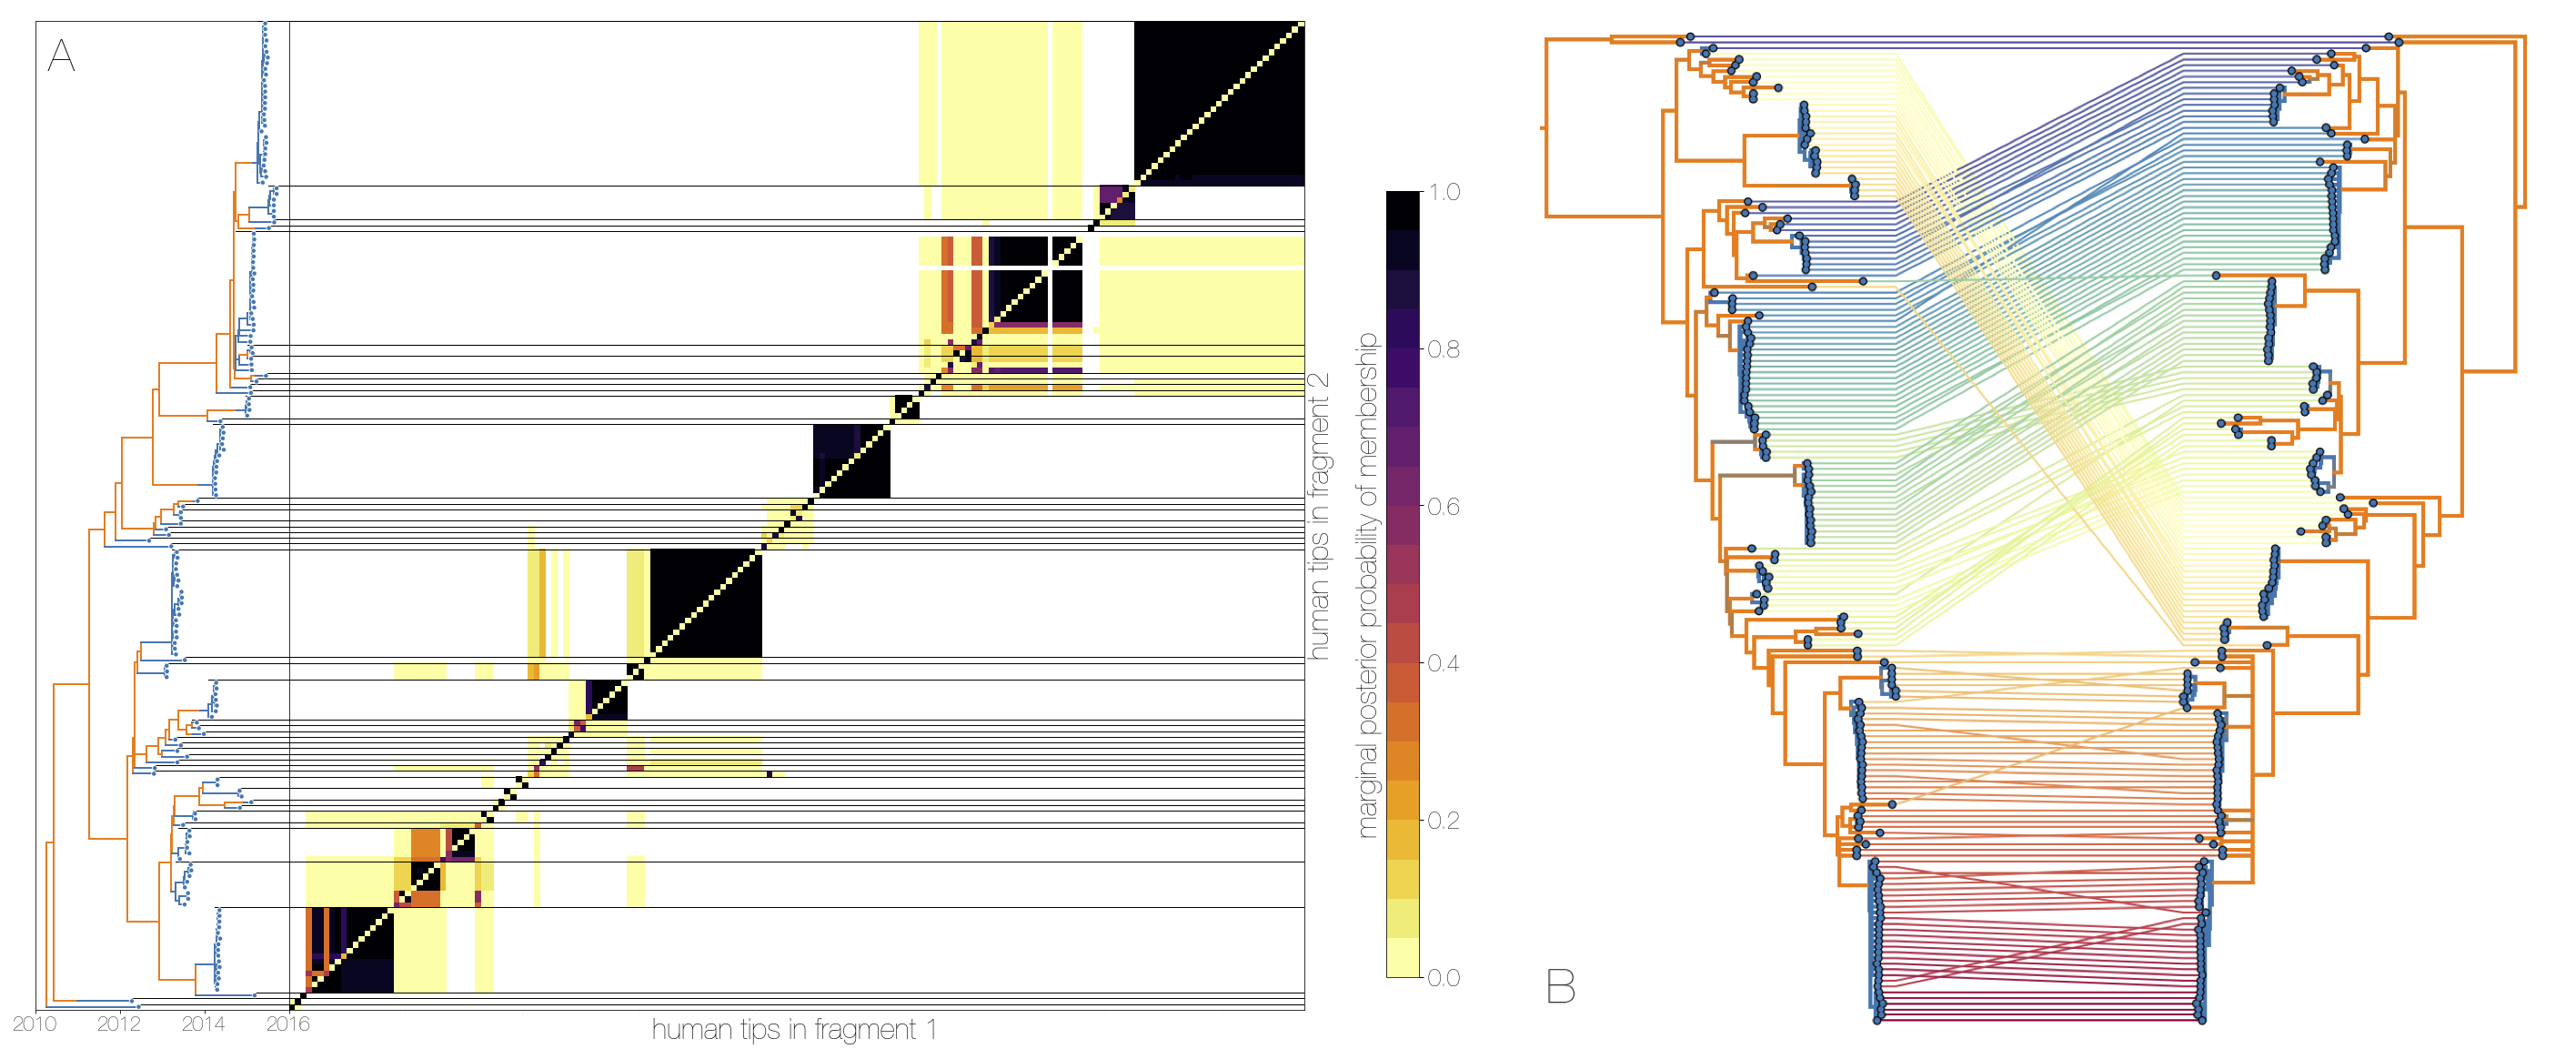
\includegraphics[width=0.95\textwidth]{figures/mers_recombinant_features.png}
    \caption{\textbf{Recombinant features of MERS-CoV phylogenies.}
    A) Heatmap showing the posterior probability that viruses from trees of different genomic fragments belong to the same introduction event.
    Genomic fragment 1 represents nucleotide positions 1 to 21000 and genomic fragment 2 represents nucleotide positions 21001 to 29364.
    The same set of viruses are arrayed on the $x$-axis and on the $y$-axis; the $x$-axis shows identity of these viruses along genomic fragment 1 and the $y$-axis shows identity of these viruses along genomic fragment 2.
    Viruses are ordered by their appearance in tree of genomic fragment 2 reduced to just the human tips and coloured by inferred host (blue for human, orange for camel) on the left.
    Human clusters are largely well-supported as monophyletic and consistent across trees of both genomic fragments.
    B) Phylogenies derived from genomic fragment 1 (left) and genomic fragment 2 (right), reduced to just the human tips.
  	Identical taxa are connected via coloured lines with colour indicating vertical position in the tree on the right.
  	Branches are coloured by inferred ancestral host state (human in blue, camel in orange).
  	Human clusters in blue change phylogenetic positions between the trees together, with little incongruence within clusters.
  	This is evidence for recombinant viruses generated in the camel reservoir entering human populations.
    }
    \label{recombinant_features}
\end{figure}

\subsection*{MERS-CoV shows population turnover in camels}

Here we attempt to investigate MERS-CoV demographic patterns in the camel reservoir.
%Since MERS-CoV in humans has a distinct epidemiology
% evolves under a distinct demographic regime, %% evolves under a demographic regime?
%we split our sequence dataset based on whether sequences were collected in humans or camels.
We supplement camel sequence data with a single earliest sequence from each human cluster, treating viral diversity present in humans as a sentinel sample of MERS-CoV diversity circulating in camels.
This removes conflicting demographic signals sampled during human outbreaks, where densely sampled closely related sequences from humans could be misconstrued as evidence of demographic crash in the viral population.

Despite lack of convergence, neither of the two demographic reconstructions show evidence of fluctuations in the relative genetic diversity ($N_e \tau$) of  MERS-CoV over time (Figure \ref{skygrid}).
However, we do note that estimates of relative genetic diversity are relatively low overall, and MERS-CoV phylogeny resembles a ladder often seen in human influenza A virus phylogenies \citep{bedford_strength_2011}.
This raises the possibility that MERS-CoV populations undergo lineage turnover at a rate not often seen in other livestock viruses (\textit{e.g.} swine influenza A viruses \citep{vijaykrishna_long-term_2011}).
Part of this could be caused by MERS-CoV ability to re-infect camels previously exposed to the virus \citep{ali_systematic_2017}, which may result in a process akin to antigenic drift, where the depletion of susceptible calves leads to ever increasing selective pressure for the virus to evolve antigenically.
While this could be tested by looking for seasonally varying patterns in selection on MERS-CoV surface proteins, recombination would remain a key confounding problem.
\tbc{Include results of N and S to indicate that surface protein is evolving quickly supporting antigenic evolution. Or not, if the data says otherwise...}

\tbc{Okay for me to leave Figure \ref{skygrid} as supplementary or it can be main text. I'm happy either way. Suggest second panel showing correspondence between fragmented genome and full genome trajectories.}

% In order to disentangle distinct demographic modes within the phylogeny of MERS-CoV we split our alignment according to whether the virus was collected from camels or humans.
% For sequences collected from humans and inferred to be in the same cluster we only keep the earliest sequence, and arrive at a sequence dataset that for the most part is comprised of viral diversity present in camels, and supplemented with human sequences that are treated as sentinel samples.


\section*{Discussion}

\subsection*{MERS-CoV epidemiology}
%\lmc{Detecting?}
In this study we aimed to understand the drivers of MERS coronavirus transmission in humans and what role the camel reservoir plays in perpetuating the epidemic in the Arabian peninsula by using sequence data collected from both hosts (174 from humans and 100 from camels).
We showed that currently existing models of population structure \citep{vaughan_efficient_2014} can identify distinct demographic modes in MERS-CoV genomic data, where viruses continuously circulating in camels repeatedly jump into humans and cause small outbreaks doomed to extinction (Figures \ref{mcc}, \ref{exploded}).
This inference succeeds under different choices of priors for unknown demographic parameters (Figure \ref{prior}) and in the presence of strong biases in sequence sampling schemes (Figure \ref{mers_epi}).
From sequence data we identify at least 50 zoonotic introductions of MERS-CoV into humans from the reservoir (Figure \ref{mcc}), from which we extrapolate that hundreds more such introductions must have taken place (Figure \ref{mers_epi}).
We also looked at potential seasonality in MERS-CoV spillover into humans.
Our analyses indicated a period of three months where the odds of a sequenced spillover event are increased, with timing consistent with an enzootic amongst camel calves (Figure \ref{seasonality}).
As a result of our identification of large and asymmetric flow of viral lineages into humans we also find that the basic reproduction number for MERS-CoV in humans is well below the epidemic threshold (Figure \ref{mers_epi}).

Strong population structure in viruses often arises through limited gene flow, either due to geography \citep{dudas_virus_2017}, ecology \citep{smith_dating_2009} or evolutionary forces \citep{turner_genomic_2005,dudas_reassortment_2015}.
On a smaller scale population structure can unveil important details about transmission patterns, such as identifying reservoirs and understanding spillover trends and risk, much as we have done here.
When properly understood naturally arising barriers to gene flow can be exploited for more efficient disease control and prevention, as well as risk management.

\subsection*{Transmissibility differences between zoonoses and pandemics}
Severe acute respiratory syndrome (SARS) coronavirus, a Betacoronavirus like MERS-CoV, caused a serious epidemic in humans in 2003, with over 8000 cases and nearly 800 deaths.
Since MERS-CoV was also able to cause significant pathogenicity in the human host it was inevitable that parallels would be drawn between MERS-CoV and SARS-CoV at the time of MERS discovery in 2012.
Although we describe the epidemiology of MERS-CoV from sequence data, indications that MERS-CoV has poor capacity to spread human-to-human existed prior to any sequence data.
SARS-CoV swept through the world in a short period of time, but MERS cases trickled slowly and were restricted to the Arabian Peninsula or resulted in self-limiting outbreaks outside of the region, a pattern strongly indicative of repeat zoonotic spillover.
Infectious disease surveillance and control measures remain limited, so much like the SARS epidemic in 2003 or the H1N1 pandemic in 2009, zoonotic pathogens with $R_{0}>1.0$ are probably going to be discovered after spreading beyond the original location of spillover.
Even though our results show that MERS-CoV does not appear to present a serious global threat, we would like to highlight that its epidemiology is nonetheless concerning.

MERS-CoV may join the list of pathogens able to jump species barriers but not spread efficiently in the new host, but every system is distinct.
Pathogens such as \textit{Bacillus anthracis}, Andes hantavirus \citep{martinez_person--person_2005}, monkeypox \citep{reed_detection_2004}, triple reassortant and H3N2v influenza A viruses \citep{shinde_triple-reassortant_2009,epperson_human_2013} belong to this list and yet only triple reassortant viruses eventually contributed to a pandemic, due to epidemiology and phylodynamics confined to influenza A virus.
When information about a system is lacking either because it is recent or entirely novel or if the system is inherently unpredictable, sequence data can and should be used jointly with whatever data sources are available to provide the unique pathogen perspective on an infectious disease outbreak.
Although MERS-CoV seems to cause self-limiting outbreaks in humans with no evidence of worsening outbreaks over time, sustained evolution of the virus in the reservoir and flow of viral lineages into humans provides the substrate for a more transmissible variant of MERS-CoV to possibly emerge.
We encourage continued genomic surveillance of MERS-CoV in the camel reservoir and from sporadic human cases.

% Despite higher resolution of inference offered by structured population models, especially when sequence data are plentiful, serious drawbacks exist.
% As the representation of evolution drifts away from a strictly bifurcating tree model, the space over which phylogenetic inference needs to take place becomes increasingly complex.
% Convergence difficulties are well known in rich models, such as ancestral recombination graphs, and multitype trees are no different.
% Even with a moderate number of sequences (N=274) and the smallest possible number of demes (N=2) structured population model mixing is slow and problematic.
% Some convergence issues (Figure \ref{skygrid}) could be attributed to the presence of recombination in MERS-CoV data (Figure \ref{recombination}), but active research into approximations to the structured coalescent \citep{maio_new_2015} seem to acknowledge both the utility and difficulties in applying such methods. %% Don't understand this sentence. How is the second clause related to the first?
% As computational infrastructure improves \citep{ayres_beagle:_2012}, %it is hopefully only a matter of time before
% phylogenetic population structure models will reach the point where large datasets with multiple demes (\textit{e.g.} West African Ebola virus epidemic \citep{dudas_virus_2017}, global influenza virus circulation \citep{bedford_global_2015}) will be tractable.

% Similar approaches have been used to quantify population structure in American Zika viruses, where repeated introductions into Florida observed in sequence data were used to extrapolate probable numbers of viral introductions


% Population structure is often inferred via phylogeny labelling approaches where discrete states are assigned to taxa, and ancestral states are reconstructed via a continuous time Markov chain the same way nucleotide sites would be.
% These methods, when used to infer ancestral migration history across a phylogeny, have thus been called ``mugration'' models.
% When the number of possible discrete states is limited, data are ample and questions are formulated well, phylogeny labelling approaches are computationally efficient, accurate and highly informative.
% However, ``mugration'' models ignore potentially relevant information, such as markedly different demographic histories in distinct populations.
%
% Sequencing of MERS-CoV has been a challenging issue, especially from the reservoir.
% MERS-CoV seroprevalence in camels, as expected of a reservoir, is very high, yet sequencing efforts have overwhelmingly focused on human infections.
% At present MERS-CoV sequences collected from humans outnumber those from camels at a ratio of over 2-to-1, and sequences from camels appear late in the MERS epidemic, largely because of the time taken to identify camels as the reservoir.
% Hence, using MERS-CoV sequence data in ``mugration'' models have led to contradictory findings, such as inference of MERS-CoV as a repeated epizootic in camels of largely human origins \citep{zhang_evolutionary_2016}.
% Traditional epidemiological approaches fare no better, since links between human cases outside of known family clusters or hospital outbreaks are exceedingly difficult to establish \citep{cauchemez_unraveling_2016}.
%
% Our study has shown how significantly different demographic regimes between hosts such as those observed in MERS-CoV can be leveraged against biased sequence data to arrive at conclusions perfectly in line with prior observations.
% MERS-CoV sequences collected from camels are, on average, relatively distantly related to each other, while human outbreaks fall into densely sampled clusters of no apparent relation to each other and of no consequence to further evolution of the virus.
% These hallmarks of distinct demographic modes were easily picked up by the explicit population structure model we employ, and reveals a cohesive picture of MERS-CoV epidemiology in agreement with previous empirical studies.
% However, we do note that at present phylogenetic models with population structure are limited in terms of computational efficiency than current models, even when approximations are used.

% \subsection*{Issues with recombination}
% Recombination in MERS-CoV is now an accepted feature of the system.
% Prevalent recombination can seriously impede phylogenetic and other sequence analysis techniques.
% We argue that although MERS-CoV sequences contain overwhelming evidence for recombination, we do not expect humans to play a major role in this process.
% As human infection with MERS-CoV remains very low, every introduction of the virus into a human population is expected to establish a clonally evolving and short-lived population.
% However, lineages crossing the species barrier are very likely to have experienced recombination at some point in their past, in some cases occurring right before zoonotic transmission, as was the case in the Korean outbreak of MERS.
% We thus conclude that while sequence analyses of MERS-CoV are perfectly legitimate for well-defined human outbreaks, extreme care must be taken when inferring their origins in the context of the reservoir, or even when comparing related outbreaks in humans.
% We also strongly advise against drawing hasty conclusions from MERS-CoV phylogenies recovered from human sequences if they span more than four months of evolution or camel sequences under virtually all circumstances, as there is no guarantee that phylogenies will cover the clonal evolutionary history of the virus in humans.

% \subsection*{Sequence data as a universal epidemiology tool} %% Drop this paragraph and finish on something better. I think this point has been made already.
% As the field of epidemiology enters the age of genomics sequence data are likely to be brought in to reinforce and augment epidemiological investigations.
% At a relatively low price, sequence data offer the combined benefits of diagnostics and typing, while also offering insight into a pathogen's evolutionary history.
% With a small amount of metadata, primarily collection dates and features of interest, such as location or host, much can be revealed through phylogenetic clustering of sequences, or absence thereof.
% This was used to great effect at all stages of the Ebola virus epidemic in West Africa, where sequence data early on were used to show continued circulation of the same strain in the region rather than multiple zoonotic introductions \citep{gire_genomic_2014}, to study viral migration at a broad level \citep{park_ebola_2015,ladner_evolution_2015} as healthcare infrastructure was being overwhelmed during the peak, and towards the end where the final transmission chains were tracked and confirmed as such \citep{arias_rapid_2016}.
% %Although sequence data can be collected for multiple reasons and used to address different questions, sequence data are a fundamental unit of ground truth, which allows sequences from wildly different studies to be combined trivially%\lmc{TRIVIALLY???} \gdc{yes, since you literally just put sequences into the same alignment}  %% AR - sorry, I hate this sentence - 'fundamental unit of ground truth' WTF?
% In fact it has often been the combination of data from distinct populations and different time periods that yielded most insight in the past \citep{dudas_virus_2017}.

%% AR - this paper is about MERS epidemiology. Finish on MERS epidemiology. The last 3 paragraphs are discussion about methods. For a high impact general journal like eLif, need to talk about the implications of the findings. Or send it to MBE.

\newpage

\section*{Methods}
\subsection*{Sequence data}
All MERS-CoV sequences were downloaded from GenBank and accession numbers are given in Table \ref{sequences}.
Sequences without accessions were kindly shared by Ali M. Somily, Mazin Barry, Sarah S. Al Subaie, Abdulaziz A. BinSaeed, Fahad A. Alzamil, Waleed Zaher, Theeb Al Qahtani, Khaldoon Al Jerian, Scott J.N. McNabb, Imad A. Al-Jahdali, Ahmed M. Alotaibi, Nahid A. Batarfi, Matthew Cotten, Simon J. Watson, Spela Binter, and Paul Kellam prior to publication.
Fragments of some strains submitted to GenBank as separate accessions were assembled into a single sequence.
Only sequences covering at least 50\% of MERS-CoV genome were kept.
Sequences were annotated with available collection dates and hosts, designated as camel or human and aligned with MAFFT \citep{katoh_mafft_2013} and edited manually.
Protein coding sequences were extracted and concatenated, reducing alignment length from 30130 down to 29364.
The final dataset consisted of 174 genomes from human infections and 100 genomes from camel infections (Table \ref{sequences}).

\subsection*{Structured coalescent analyses}

For our primary analysis, the MultiTypeTree module \citep{vaughan_efficient_2014} of BEAST v2.4.3 \citep{bouckaert_beast_2014} was used to specify a structured coalescent model with two demes -- humans and camels.
This model estimates 4 parameters: rate of coalescence in human viruses, rate of coalescence in camel viruses, rate of migration from the human deme to the camel deme and rate of migration from the camel deme to the human deme.
Analyses were run on codon position partitioned data with two separate HKY+$\Gamma_{4}$ \citep{hky_1985,yang_1994} nucleotide substitution models specified for codon positions 1+2 and 3.
A relaxed molecular clock with branch rates drawn from a lognormal distribution \citep{drummond_2006} was used to infer the evolutionary rate from date calibrated tips.
Default priors were used for all parameters except for migration rates between demes for which an exponential prior with mean 1.0 was used.
All analyses were run for 200 million steps across ten independent Markov chains (MCMC runs) and states were sampled every \tbc{XXX} steps.
Due to the complexity of multitype tree parameter space 50\% of states from every analysis were discarded as burn-in, convergence assessed in Tracer v1.6 and states combined using LogCombiner distributed with BEAST v2.4.3 \citep{bouckaert_beast_2014}.
Three chains out of ten did not converge and were discarded altogether.
This left \tbc{XXX} states on which to base posterior inference.

As a secondary analysis to test robustness to choice of prior, we set up an analysis where we increased the mean of the exponential distribution prior for migration rate to 10.0.
All other parameters were identical to the primary analysis and as before 10 independent MCMC chains were run.
In this case, two chains did not converge.
This left \tbc{XXX} states on which to base posterior inference.

As an additional secondary analysis, we also considered a scenario where alignments were split into two fragments (fragment 1 comprised of positions 1-21000, fragment 2 of positions 21000-onwards), with independent clocks, trees and migration rates, but shared substitution models and deme population sizes.
Fragment positions were chosen based on consistent identification of the region around nucleotide 21000 as a probable breakpoint by GARD \citep{pond_gard:_2006} by previous studies into SARS and MERS coronaviruses \citep{hon_evidence_2008,dudas_mers-cov_2016}.
All analyses were set to run for 200 million states, subsampling every 20 000 states.
Chains not converging after 200 million states were discarded.
20\% of the states were discarded as burn-in, convergence assessed with Tracer 1.6 and combined with LogCombiner.
Three chains out of ten did not converge.
This left \tbc{XXX} states on which to base posterior inference.

\subsubsection*{Introduction seasonality}

We extracted the times of camel-to-human introductions from the posterior distribution of multitype trees.
This distribution of introduction times was then discretised as follows: for sample  $k = 1, 2, \ldots, L$ from the posterior,  $Z_{ijk}$ was $1$ if there as an introduction in month $i$ and year $j$ and $0$ otherwise.
We model the variable $Y_{ij} = \sum_{k = 1}^L Z_{ijk}$ with the hierarchical model:
\begin{align*}
  Y_{ij} &\sim \text{Binomial}(L, \theta_{ij}); \\
  logit(\theta_{ij}) &= \alpha_j + \beta_i; \\
  \beta_i &\sim \text{Normal}(0, \sigma_{m}); \\
  \sigma_{m} &\sim \text{Cauchy}(0, 2.5); \\
  \alpha_j &\sim \text{Normal}(\mu_{y}, \sigma_{y}); \\
  \mu_{y}  &\sim  \text{Normal}(0, 1); \\
  \sigma_{y} &\sim \text{Cauchy}(0, 2.5).
\end{align*}

Odds ratios of introductions can then be computed for each month $i$ as $\text{OR}_i = \exp(\beta_i)$.
\tbc{Please spell out what parameters are referring to. In English, what is $\alpha_j$ and what is $\beta_i$? I'm having a hard time figuring out what's going on here.}
\tbc{Can you move `\textit{logit}' to the right hand side of the equation (if not too messy)?}

\subsection*{Epidemiological analyses}

As of 10 May 2017, the World Health Organization has been notified of 1952 cases of MERS-CoV.
We thus simulate final transmission chain sizes using equation \ref{clusterLikelihood} \citep{lloyd-smith_superspreading_2005,blumberg_inference_2013} until we reach an epidemic comprised of 2000 cases.
10 000 simulations were run for 121 uniformly spaced values of R$_{0}$ across the range [0.5--1.1] with dispersion parameter $\omega$ fixed to 0.1.
Each simulation results in a vector of outbreak sizes $C$, where $C_{i}$ is the size of the \textit{i}th transmission cluster and $\sum_{i=1}^{K} C_{i} = 2000$, where $K$ is the number of clusters generated.
We sample from the case cluster size vector according to a multivariate hypergeometric distribution to simulate sequencing (algorithm \ref{hypergeometric}).
The resulting sequence cluster size vector $S$ contains $K$ entries, some of which are zero (\textit{i.e.} case clusters not sequenced), but $\sum_{i=1}^{K} S_{i} = 174$ which reflects the number of MERS-CoV sequences used in this study.
Since the sampling scheme operates under equi-probable sequencing we also simulated biased sequencing by using concentrated hypergeometric distributions where the probability mass function is squared (bias = 2) or cubed (bias = 3) and then normalized.
This makes clusters likely to be `sequenced' even more likely to be sequenced and \textit{vice versa}.
We performed a smaller set of simulations with 2500 replicates and twice the number of cases, \textit{i.e.} $\sum_{i=1}^{K} C_{i} = 4000$, to explore a dramatically underreported epidemic.

Let $R_{0}$ be the basic reproductive number ($ 0 < R_{0} < 1$),  and $\omega > 0$ be the a dispersion parameter, then the probability of observing a stuttering chain (cluster) $r$ of size $j$ is~\citep{blumberg_inference_2013}
\begin{equation}
Pr(r = j | R_{0}, \omega) = \frac{\Gamma(\omega j+j-1)}{\Gamma(\omega j)\Gamma(j+1)} \frac{(\frac{R_{0}}{\omega})^{j-1}}{(1+\frac{R_{0}}{\omega})^{\omega j+j-1}}.
\label{clusterLikelihood}
\end{equation}

Although case clusters and their sizes are difficult to infer directly and require detailed epidemiological follow up, sequence data have fewer limitations.%\lmc{other than the ``obvious'' limitation that they're \textbf{not} the actual infection process, uh? >.>} \gdc{fair point, but we're talking about cluster inference}
Our structured coalescent analyses indicate that every MERS outbreak is a contained cross-species transmission of the virus from camels into humans.
The distribution of the number of these cross-species transmissions and their sizes thus contain information about the underlying distribution of case clusters.
We employ a Monte Carlo simulation approach to identify simulations where the recovered distribution of sequence cluster sizes fall within the 95\% highest posterior density intervals for three summary statistics of MERS-CoV sequence cluster sizes recovered via structured coalescent analyses: mean, median and standard deviation.
These values are 2.90--3.70 for mean sequence cluster size, 4.87--6.07 for standard deviation of sequence cluster sizes and a median sequence cluster size of 1.

\begin{algorithm}[H]
 \KwData{Array of case cluster sizes in outbreak $\boldsymbol C = [C_{1},C_{2}, \ldots, C_{K}]$, sequences available $M$, total outbreak size $\sum_{i=1}^{K} C_{i}$.}
 \KwResult{Array of sequence cluster sizes sampled: $\boldsymbol S = [S_{1},S_{2}, \ldots, S_{K}]$.}
 Draw $S_{i}$ from a hypergeometric distribution with $C_{i}$ successes, $\sum_{i=1}^{K} C_{i}-C_{i}$ failures after $M$ trials\;
 \While{$i < K$}{
  $i = i + 1$\;
  $M = M - S_{i-1}$\;
  Compute the probability mass function (pmf) for all possible values of $S_i$, $\boldsymbol p = [p(0)^{\text{bias}}, p(1)^{\text{bias}}, \ldots, p(C_{i})^{\text{bias}}] \times (\sum_i p_i^{\text{bias}}) ^{-1}$, where $p(\cdot)$  is the pmf for a hypergeometric distribution with $C_{i}$ successes, $\sum_{i=1}^{K} C_{i}-C_{i}$ failures after $M$ trials\;
  Draw a sequence cluster size $S_{i}$ from array of potential sequence cluster sizes $[0, 1, \ldots, C_{i}]$ according to $\boldsymbol p$\;
 }
 Add remaining sequences to last sequence cluster $C_{K} = M - S_{K-1}$\;
 \caption{\textbf{Multivariate hypergeometric sampling scheme.}
 Pseudocode describes the multivariate hypergeometric sampling scheme that simulates sequencing.
 Probability of sequencing a given number of cases from a case cluster depends on cluster size and sequences left (\textit{i.e.} ``sequencing capacity'').
 The bias parameter determines how probability mass function of the hypergeometric distribution is concentrated.
 }
 \label{hypergeometric}
\end{algorithm}

\subsection*{Demographic inference of MERS-CoV in the reservoir}
In order to infer the demographic history of MERS-CoV in camels we used the results of structured coalescent analyses to identify introductions of the virus into humans.
The oldest sequence from each cluster introduced into humans was used to represent a random draw from the diversity of MERS-CoV circulating in camels.
These sequences were combined with existing sequence data from camels to give us a dataset with minimal demographic signal coming from epidemiological processes in humans.
Sequences belonging to the outgroup clade where most of MERS-CoV sequences from Egypt fall were removed out of concern that MERS epidemics in the Arabian Peninsula and Egypt are distinct epidemics with relatively poor sampling in the latter.
A flexible skygrid tree prior \citep{gill_2013} was used to recover estimates of relative genetic diversity ($N_{e}\tau$) at 50 evenly spaced grid points across six years, ending at the most recent tip in the tree (2015 August) in BEAST v1.8.4 \citep{drummond_bayesian_2012}.
We set up five independent MCMC chains to run for 500 million states, sampling every 50 000 states.
This analysis suffered from poor convergence, where two chains converged onto one stationary distribution, two to another and the last chain onto a third stationary distribution, with high effective sample sizes.
Demographic trajectories recovered by the two main stationary distributions are very similar and differences between the two appear to be caused by convergence onto different tree topologies, with onward effects on evolutionary rate estimates and distributions of coalescence times.
\tbc{This statement seemd a bit strong, as it looked like the $N_{e}\tau$ trajectory was highly similar between these different stationary distributions.}
This non-convergence effect may have been masked previously by the use of all available MERS-CoV sequences from humans which may have lead MCMC towards one of the multiple stationary distributions.

\subsection*{Data availability}
Sequence data and all analytical code is publicly available at \href{https://github.com/blab/structured-mers}{github.com/blab/structured-mers}.

\section*{Acknowledgements}
We would like to thank Allison Black for useful discussion and advice.
GD is supported by the Mahan postdoctoral fellowship from the Fred Hutchinson Cancer Research Center.
TB is a Pew Biomedical Scholar and is supported by NIH R35 GM119774-01.
We gratefully acknowledge the contribution of the following scientists for sharing MERS-CoV sequence data before publication:

Ali M. Somily$^{1}$, Mazin Barry$^{1}$, Sarah S. Al Subaie$^{1}$, Abdulaziz A. BinSaeed$^{1}$, Fahad A. Alzamil$^{1}$, Waleed Zaher$^{1}$, Theeb Al Qahtani$^{1}$, Khaldoon Al Jerian$^{1}$, Scott J.N. McNabb$^{2}$, Imad A. Al-Jahdali$^{3}$, Ahmed M. Alotaibi$^{4}$, Nahid A. Batarfi$^{5}$, Matthew Cotten$^{6}$, Simon J. Watson$^{6}$, Spela Binter$^{6}$, Paul Kellam$^{6}$.


$^{1}$College of Medicine, King Saud University, Riyadh, Kingdom of Saudi Arabia \\
$^{2}$Rollins School of Public Health, Emory University, Atlanta, GA, USA \\
$^{3}$Deputy Minister. Ex. General Director King Fahad General Hospital, Jeddah and Occupational and environmental medicine, Um AlQura University, Kingdom of Saudi Arabia \\
$^{4}$Department of Intensive Care, Prince Mohammed bin Abdulaziz Hospital, Riyadh, Kingdom of Saudi Arabia \\
$^{5}$Epidemiology section, Command and Control Center (CCC) Ministry of Health, Jeddah \\
$^{6}$Wellcome Trust Sanger Institute, Hinxton, United Kingdom \\


\bibliographystyle{mbe}
\bibliography{mers-structure}

\newpage

\setcounter{figure}{0}
\setcounter{table}{0}
\renewcommand{\thefigure}{S\arabic{figure}}
\renewcommand{\thetable}{S\arabic{table}}

\begin{longtable}{ | r | l | p{2cm} | l | l | }

  \caption{Strain names, accessions (where available), identified host and reported collection dates for MERS-CoV genomes used in this study.} \label{sequences} \\


  \hline & strain & accession & host & collection date \\ \hline
  \endfirsthead

  \multicolumn{5}{l}%
  {{\bfseries \tablename\ \thetable{} -- continued from previous page}} \\

  \hline & strain & accession & host & collection date \\ \hline
  \endhead

  \hline \multicolumn{5}{|r|}{{Continued on next page}} \\ \hline
  \endfoot

  \hline \hline
  \endlastfoot

  1 & KSA-378 & KJ713296 & camel & 2013-11 \\
  2 & KSA-363 & KJ713298 & camel & 2013-11 \\
  3 & KSA-503 & KJ713297 & camel & 2013-11 \\
  4 & KSA-376 & KJ713299 & camel & 2013-11 \\
  5 & KSA-505 & KJ713295 & camel & 2013-11 \\
  6 & Jeddah-1 & KF917527 & camel & 2013-11-08 \\
  7 & NRCE-HKU205 & KJ477102 & camel & 2013-11-15 \\
  8 & KFU-HKU1 & KJ650297 & camel & 2013-11-30 \\
  9 & KFU-HKU13 & KJ650295 & camel & 2013-12-30 \\
  10 & Camel\_Egypt\_NRCE-HKU271 &  & camel & 2013-12-30 \\
  11 & Camel\_Egypt\_NRCE-HKU270 &  & camel & 2013-12-30 \\
  12 & KFU-HKU19Dam & KJ650296 & camel & 2013-12-30 \\
  13 & Qatar\_2\_2014 & KJ650098 & camel & 2014-02-16 \\
  14 & UAE/D469-14 & KU242424 & camel & 2014-03-04 \\
  15 & UAE/D511-14 & KU242423 & camel & 2014-03-12 \\
  16 & Jeddah/F13A/2014 & KT368824 & camel & 2014-05 \\
  17 & UAE/D1164.10/2014 & KP719928 & camel & 2014-06 \\
  18 & UAE/D1339.2/2014 & KP719931 & camel & 2014-06 \\
  19 & UAE/D1164.11/2014 & KP719929 & camel & 2014-06 \\
  20 & UAE/D1164.9/2014 & KP719927 & camel & 2014-06 \\
  21 & UAE/D1209/2014 & KP719933 & camel & 2014-06 \\
  22 & UAE/D1164.14/2014 & KP719930 & camel & 2014-06 \\
  23 & UAE/D1243.12/2014 & KP719932 & camel & 2014-06 \\
  24 & D1164.1/14 & KX108937 & camel & 2014-06-02 \\
  25 & Riyadh/Ry23N/2014 & KT368825 & camel & 2014-07 \\
  26 & Riyadh/Ry84N/2014 & KT368826 & camel & 2014-07 \\
  27 & Jeddah/S93/2014 & KT368855 & camel & 2014-09 \\
  28 & Jeddah/401/2014 & KT368827 & camel & 2014-09 \\
  29 & Jeddah/S100/2014 & KT368853 & camel & 2014-09 \\
  30 & Jeddah/S99/2014 & KT368857 & camel & 2014-09 \\
  31 & Jeddah/S94/2014 & KT368856 & camel & 2014-09 \\
  32 & Jeddah/S73/2014 & KT368854 & camel & 2014-09 \\
  33 & Jeddah/O47b/2014 & KT368852 & camel & 2014-10 \\
  34 & Jeddah/O23b/2014 & KT368849 & camel & 2014-10 \\
  35 & Jeddah/O24/2014 & KT368850 & camel & 2014-10 \\
  36 & Jeddah/O30/2014 & KT368851 & camel & 2014-10 \\
  37 & Jeddah/N51/2014 & KT368846 & camel & 2014-11 \\
  38 & Jeddah/N68b/2014 & KT368848 & camel & 2014-11 \\
  39 & Jeddah/N62b/2014 & KT368847 & camel & 2014-11 \\
  40 & Jeddah/D40/2014 & KT368834 & camel & 2014-12 \\
  41 & Jeddah/D90/2014 & KT368844 & camel & 2014-12 \\
  42 & Jeddah/D88/2014 & KT368843 & camel & 2014-12 \\
  43 & Jeddah/D36/2014 & KT368832 & camel & 2014-12 \\
  44 & Jeddah/D35/2014 & KT368831 & camel & 2014-12 \\
  45 & Jeddah/D92/2014 & KT368845 & camel & 2014-12 \\
  46 & Jeddah/D49/2014 & KT368841 & camel & 2014-12 \\
  47 & Jeddah/D34/2014 & KT368830 & camel & 2014-12 \\
  48 & Jeddah/D33b/2014 & KT368829 & camel & 2014-12 \\
  49 & Jeddah/D42/2014 & KT368835 & camel & 2014-12 \\
  50 & Jeddah/D50b/2014 & KT368842 & camel & 2014-12 \\
  51 & Jeddah/D45/2014 & KT368837 & camel & 2014-12 \\
  52 & Jeddah/D46b/2014 & KT368838 & camel & 2014-12 \\
  53 & Jeddah/D43b/2014 & KT368836 & camel & 2014-12 \\
  54 & Jeddah/D100/2014 & KT368828 & camel & 2014-12 \\
  55 & Jeddah/D47/2014 & KT368839 & camel & 2014-12 \\
  56 & Jeddah/D38b/2014 & KT368833 & camel & 2014-12 \\
  57 & Jeddah/D48/2014 & KT368840 & camel & 2014-12 \\
  58 & D2597.2/14 & KX108938 & camel & 2014-12-13 \\
  59 & Egypt\_NRCE-NC163/2014 & KU740200 & camel & 2014-12-17 \\
  60 & Jeddah/Jd7/2015 & KT368861 & camel & 2015-01 \\
  61 & Jeddah/Jd86/2015 & KT368863 & camel & 2015-01 \\
  62 & Jeddah/Jd90/2015 & KT368865 & camel & 2015-01 \\
  63 & Jeddah/Jd1b/2015 & KT368858 & camel & 2015-01 \\
  64 & Jeddah/Jd4/2015 & KT368859 & camel & 2015-01 \\
  65 & Jeddah/Jd85/2015 & KT368862 & camel & 2015-01 \\
  66 & Jeddah/Jd6b/2015 & KT368860 & camel & 2015-01 \\
  67 & Jeddah/Jd87/2015 & KT368864 & camel & 2015-01 \\
  68 & D252/15 & KX108939 & camel & 2015-01-30 \\
  69 & Jeddah/Jd199/2015 & KT368867 & camel & 2015-02 \\
  70 & Jeddah/Jd175/2015 & KT368866 & camel & 2015-02 \\
  71 & D374/15 & KX108940 & camel & 2015-02-12 \\
  72 & D383/15 & KX108941 & camel & 2015-02-14 \\
  73 & D389/15 & KX108942 & camel & 2015-02-15 \\
  74 & Riyadh/Ry63/2015 & KT368876 & camel & 2015-03 \\
  75 & Riyadh/Ry136/2015 & KT368868 & camel & 2015-03 \\
  76 & Riyadh/Ry178/2015 & KT368874 & camel & 2015-03 \\
  77 & Riyadh/Ry162/2015 & KT368871 & camel & 2015-03 \\
  78 & Riyadh/Ry86/2015 & KT368879 & camel & 2015-03 \\
  79 & Taif/T150/2015 & KT368889 & camel & 2015-03 \\
  80 & Riyadh/Ry137/2015 & KT368869 & camel & 2015-03 \\
  81 & Riyadh/Ry179/2015 & KT368875 & camel & 2015-03 \\
  82 & Riyadh/Ry177/2015 & KT368873 & camel & 2015-03 \\
  83 & Riyadh/Ry79/2015 & KT368878 & camel & 2015-03 \\
  84 & Riyadh/Ry173/2015 & KT368872 & camel & 2015-03 \\
  85 & Taif/T157b/2015 & KT368890 & camel & 2015-03 \\
  86 & Riyadh/Ry159b/2015 & KT368870 & camel & 2015-03 \\
  87 & Riyadh/Ry64/2015 & KT368877 & camel & 2015-03 \\
  88 & Taif/T3/2015 & KT368880 & camel & 2015-04 \\
  89 & Taif/T16/2015 & KT368882 & camel & 2015-04 \\
  90 & Taif/T22/2015 & KT368883 & camel & 2015-04 \\
  91 & Taif/T92/2015 & KT368887 & camel & 2015-04 \\
  92 & Taif/T7/2015 & KT368881 & camel & 2015-04 \\
  93 & Taif/T91b/2015 & KT368886 & camel & 2015-04 \\
  94 & Taif/T68/2015 & KT368884 & camel & 2015-04 \\
  95 & Taif/T89/2015 & KT368885 & camel & 2015-04 \\
  96 & Taif/T98/2015 & KT368888 & camel & 2015-04 \\
  97 & D998/15 & KX108943 & camel & 2015-04-23 \\
  98 & D1157/15 & KX108944 & camel & 2015-05-12 \\
  99 & D1189.1/15 & KX108946 & camel & 2015-05-18 \\
  100 & D1271/15 & KX108945 & camel & 2015-05-29 \\
  101 & Jordan-N3/2012 & KC776174 & human & 2012-04-15 \\
  102 & EMC/2012 & JX869059 & human & 2012-06-13 \\
  103 & England/1/2012 & KC164505 & human & 2012-09-11 \\
  104 & Riyadh\_1\_2012 & KF600612 & human & 2012-10-23 \\
  105 & Riyadh\_2\_2012 & KF600652 & human & 2012-10-30 \\
  106 & Riyadh\_3\_2013 & KF600613 & human & 2013-02-05 \\
  107 & England/3/2013 & KM210278 & human & 2013-02-10 \\
  108 & England/2/2013 & KM015348 & human & 2013-02-10 \\
  109 & England/4/2013 & KM210277 & human & 2013-02-13 \\
  110 & Riyadh\_4\_2013 & KJ156952 & human & 2013-03-01 \\
  111 & Munich/AbuDhabi/2013 & KF192507 & human & 2013-03-22 \\
  112 & Al-Hasa\_2\_2013 & KF186566 & human & 2013-04-21 \\
  113 & Al-Hasa\_3\_2013 & KF186565 & human & 2013-04-22 \\
  114 & UAE-FRA1\_1627-2013\_BAL & KJ361500 & human & 2013-04-26 \\
  115 & Al-Hasa\_4\_2013 & KF186564 & human & 2013-05-01 \\
  116 & Al-Hasa\_7\_2013 & KF600623, KF600655 & human & 2013-05-01 \\
  117 & Al-Hasa\_8\_2013 & KF600618, KF600626, KF600635, KF600638 & human & 2013-05-01 \\
  118 & Al-Hasa\_25\_2013 & KJ156866 & human & 2013-05-02 \\
  119 & Al-Hasa\_11\_2013 & KF600629, KF600636, KF600646 & human & 2013-05-03 \\
  120 & Al-Hasa\_12\_2013 & KF600627 & human & 2013-05-07 \\
  121 & Al-Hasa\_14\_2013 & KF600615, KF600643 & human & 2013-05-08 \\
  122 & Al-Hasa\_1\_2013 & KF186567 & human & 2013-05-09 \\
  123 & Al-Hasa\_15\_2013 & KF600645 & human & 2013-05-11 \\
  124 & Al-Hasa\_16\_2013 & KF600644 & human & 2013-05-12 \\
  125 & Buraidah\_1\_2013 & KF600630 & human & 2013-05-13 \\
  126 & Al-Hasa\_23\_2013 & KJ156860, KJ156894, KJ156929, KJ156923, KJ156862 & human & 2013-05-13 \\
  127 & Al-Hasa\_17\_2013 & KF600647 & human & 2013-05-15 \\
  128 & Al-Hasa\_19\_2013 & KF600632 & human & 2013-05-23 \\
  129 & Al-Hasa\_18\_2013 & KF600651 & human & 2013-05-23 \\
  130 & Al-Hasa\_21\_2013 & KF600634 & human & 2013-05-30 \\
  131 & Hafr-Al-Batin\_1\_2013 & KF600628 & human & 2013-06-04 \\
  132 & Wadi-Ad-Dawasir\_1\_2013 & KJ156881 & human & 2013-06-12 \\
  133 & Taif\_1\_2013 & KJ156949 & human & 2013-06-12 \\
  134 & Taif\_2\_2013 & KJ156896, KJ156876 & human & 2013-06-12 \\
  135 & Taif\_3\_2013 & KJ156938, KJ156897, KJ156922, KJ156868, KJ156921, KJ156915,
KJ156906 & human & 2013-06-13 \\
  136 & Al-Hasa\_26\_2013 & KJ156882, KJ156941, KJ156872 & human & 2013-06-18 \\
  137 & Al-Hasa\_27\_2013 & KJ156943, KJ156939 & human & 2013-06-19 \\
  138 & Al-Hasa\_28\_2013 & KJ156887, KJ156940, KJ156889, KJ156893, KJ156884, KJ156930,
KJ156928, KJ156909 & human & 2013-06-22 \\
  139 & Riyadh\_6\_2013 & KJ156879, KJ156947, KJ156890, KJ156908, KJ156927 & human & 2013-07-02 \\
  140 & Riyadh\_5\_2013 & KJ156944 & human & 2013-07-02 \\
  141 & Riyadh\_7\_2013 & KJ156937, KJ156905 & human & 2013-07-15 \\
  142 & Riyadh\_8\_2013 & KJ156880, KJ156942 & human & 2013-07-17 \\
  143 & Riyadh\_9\_2013 & KJ156869 & human & 2013-07-17 \\
  144 & Hafr-Al-Batin\_2\_2013 & KJ156910 & human & 2013-08-05 \\
  145 & Asir\_2\_2013 & KJ156863, KJ156899, KJ156912, KJ156900, KJ156898, KJ156945,
KJ156932 & human & 2013-08-05 \\
  146 & Riyadh\_11\_2013 & KJ156946, KJ156911 & human & 2013-08-06 \\
  147 & Riyadh\_12\_2013 & KJ156926, KJ156901 & human & 2013-08-08 \\
  148 & Riyadh\_13\_2013 & KJ156888, KJ156873 & human & 2013-08-13 \\
  149 & Riyadh\_14\_2013 & KJ156934 & human & 2013-08-15 \\
  150 & Hafr-Al-Batin\_4\_2013 & KJ156931, KJ156895, KJ156864, KJ156861 & human & 2013-08-25 \\
  151 & Hafr-Al-Batin\_5\_2013 & KJ156951, KJ156924, KJ156954, KJ156913 & human & 2013-08-25 \\
  152 & Riyadh\_17\_2013 & KJ156918, KJ156920, KJ156865 & human & 2013-08-26 \\
  153 & Hafr-Al-Batin\_6\_2013 & KJ156874 & human & 2013-08-28 \\
  154 & Riyadh\_10\_2013 & KJ156891, KJ156936, KJ156907 & human & 2013-09-05 \\
  155 & Madinah\_3b\_2013 & KJ156950, KJ156916 & human & 2013-09-11 \\
  156 & Qatar3 & KF961221 & human & 2013-10-13 \\
  157 & Qatar4 & KF961222 & human & 2013-10-17 \\
  158 & Oman\_2285\_2013 & KT156560 & human & 2013-10-28 \\
  159 & Jeddah-1 & KF958702 & human & 2013-11-05 \\
  160 & AbuDhabi\_UAE\_9\_2013 & KP209312 & human & 2013-11-15 \\
  161 & Oman\_2874\_2013 & KT156561 & human & 2013-12-28 \\
  162 & AbuDhabi/Gayathi\_UAE\_2\_2014 & KP209310 & human & 2014-03-07 \\
  163 & Jeddah\_C7569/KSA & KM027256 & human & 2014-04-03 \\
  164 & Jeddah\_C7149/KSA & KM027255 & human & 2014-04-05 \\
  165 & Jeddah\_C7770/KSA & KM027257 & human & 2014-04-07 \\
  166 & AbuDhabi\_UAE\_8\_2014 & KP209306 & human & 2014-04-07 \\
  167 & AbuDhabi\_UAE\_16\_2014 & KP209308 & human & 2014-04-10 \\
  168 & AbuDhabi\_UAE\_18\_2014 & KP209307 & human & 2014-04-10 \\
  169 & Jeddah\_C8826/KSA & KM027258 & human & 2014-04-12 \\
  170 & AbuDhabi\_UAE\_26\_2014 & KP209313 & human & 2014-04-13 \\
  171 & Jeddah\_C9055/KSA & KM027259 & human & 2014-04-14 \\
  172 & Makkah\_C9355/KSA/Makkah & KM027261 & human & 2014-04-15 \\
  173 & AbuDhabi\_UAE\_33\_2014 & KP209311 & human & 2014-04-17 \\
  174 & AbuDhabi\_UAE\_30\_2014 & KP209309 & human & 2014-04-19 \\
  175 & Jeddah\_C10306/KSA & KM027260 & human & 2014-04-21 \\
  176 & Riyadh\_2014KSA\_683/KSA/2014 & KM027262 & human & 2014-04-22 \\
  177 & Riyadh-KKUH-90b &  & human & 2014-04-24 \\
  178 & Riyadh-KKUH-105 &  & human & 2014-04-25 \\
  179 & Riyadh-KKUH-104 &  & human & 2014-04-25 \\
  180 & KFMC-1 & KT121580 & human & 2014-04-28 \\
  181 & KFMC-8 & KT121579 & human & 2014-04-30 \\
  182 & Indiana/USA-1\_SaudiArabia\_2014 & KJ813439 & human & 2014-04-30 \\
  183 & KFMC-10 & KT121578 & human & 2014-05-01 \\
  184 & KFMC-7 & KT121581 & human & 2014-05-03 \\
  185 & Riyadh-KKUH-291 &  & human & 2014-05-06 \\
  186 & KFMC-9 & KT121574 & human & 2014-05-07 \\
  187 & KFMC-3 & KT121573 & human & 2014-05-09 \\
  188 & Florida/USA-2\_SaudiArabia\_2014 & KJ829365 & human & 2014-05-10 \\
  189 & KFMC-2 & KT121577 & human & 2014-05-11 \\
  190 & KFMC-4 & KT121575 & human & 2014-05-12 \\
  191 & KFMC-5 & KT121572 & human & 2014-05-12 \\
  192 & Riyadh-KKUH-368 &  & human & 2014-05-13 \\
  193 & KFMC-6 & KT121576 & human & 2014-05-18 \\
  194 & Riyadh\_2014KSA\_158/KSA/2014 & KM027281 & human & 2014-05-20 \\
  195 & Jeddah-KFH-285TA &  & human & 2014-06-03 \\
  196 & Jeddah-KFH-605TD &  & human & 2014-06-09 \\
  197 & Jeddah-KFH-668TD &  & human & 2014-06-09 \\
  198 & Jeddah-KFH-899NF &  & human & 2014-06-16 \\
  199 & Jeddah-KFH-949NSG1 &  & human & 2014-06-18 \\
  200 & Riyadh-KKUH-643 &  & human & 2014-11-02 \\
  201 & Taif/KSA-7032/2014 & KU710264 & human & 2014-11-04 \\
  202 & Riyadh-KKUH-665 &  & human & 2014-11-19 \\
  203 & Riyadh-KSA-2049/2015 & KR011266 & human & 2015-01-06 \\
  204 & Riyadh-KSA-2343/2015 & KR011264 & human & 2015-01-21 \\
  205 & Riyadh-KSA-2345/2015 & KR011263 & human & 2015-01-21 \\
  206 & Riyadh-KSA-2466/2015 & KR011265 & human & 2015-01-26 \\
  207 & Kharj-KSA-2599/2015 & KT806052 & human & 2015-02-02 \\
  208 & Kharj-KSA-2598/2015 & KT806053 & human & 2015-02-02 \\
  209 & Riyadh-KSA-2716/2015 & KT806051 & human & 2015-02-05 \\
  210 & Khobar-KSA-6736/2015 & KT806048 & human & 2015-02-07 \\
  211 & Jeddah-KSA-C20843/2015 & KT806044 & human & 2015-02-09 \\
  212 & Jeddah-KSA-C20860/2015 & KT806055 & human & 2015-02-10 \\
  213 & Riyadh\_KSA\_2959\_2015 & KT026453 & human & 2015-02-10 \\
  214 & Riyadh-KSA-3065/2015 & KT806050 & human & 2015-02-12 \\
  215 & Najran-KSA-C20915/2015 & KT806054 & human & 2015-02-13 \\
  216 & Riyadh-KSA-3181/2015 & KT806049 & human & 2015-02-15 \\
  217 & Riyadh\_KKUH\_0734 &  & human & 2015-02-18 \\
  218 & Jeddah-KSA-C21271/2015 & KT806045 & human & 2015-02-22 \\
  219 & Riyadh\_KKUH\_0755 &  & human & 2015-02-23 \\
  220 & Riyadh\_KKUH\_0756 &  & human & 2015-02-23 \\
  221 & Riyadh\_KKUH\_0780 &  & human & 2015-02-25 \\
  222 & Riyadh\_KKUH\_0801 &  & human & 2015-02-27 \\
  223 & Riyadh\_KKUH\_0826 &  & human & 2015-02-28 \\
  224 & Riyadh\_KKUH\_0818 &  & human & 2015-02-28 \\
  225 & Riyadh\_KSA\_4050\_2015 & KT026454 & human & 2015-03-01 \\
  226 & Riyadh\_KKUH\_0944 &  & human & 2015-03-02 \\
  227 & Riyadh\_KKUH\_0939 &  & human & 2015-03-02 \\
  228 & Riyadh\_KKUH\_1080 &  & human & 2015-03-03 \\
  229 & Riyadh\_KKUH\_1066 &  & human & 2015-03-03 \\
  230 & Riyadh\_KKUH\_1145 &  & human & 2015-03-04 \\
  231 & Riyadh\_KKUH\_1217 &  & human & 2015-03-04 \\
  232 & Riyadh\_KKUH\_1461 &  & human & 2015-03-08 \\
  233 & Riyadh\_KKUH\_1470 &  & human & 2015-03-08 \\
  234 & Riyadh\_KKUH\_1522 &  & human & 2015-03-09 \\
  235 & Germany3/UAE-Dubai/Abu-Dhabi &  & human & 2015-03-11 \\
  236 & Hufuf-KSA-9158/2015 & KT806047 & human & 2015-03-27 \\
  237 & Hufuf-KSA-11002/2015 & KT806046 & human & 2015-05-10 \\
  238 & KOR/KNIH/002\_05\_2015 & KT029139 & human & 2015-05-20 \\
  239 & ChinaGD01 & KT036372 & human & 2015-05-28 \\
  240 & KOR/Seoul/014-2015 & KX034093 & human & 2015-05-30 \\
  241 & KOREA/Seoul/014-1-2015 & KT374052 & human & 2015-05-31 \\
  242 & KOREA/Seoul/035-1-2015 & KT374054 & human & 2015-06-03 \\
  243 & KOR/Seoul/066-2015 & KX034095 & human & 2015-06-04 \\
  244 & Korea/Seoul/SNU1-035/2015 & KU308549 & human & 2015-06-08 \\
  245 & KOR/CNUH\_SNU/030\_06\_2015 & KT868868 & human & 2015-06-08 \\
  246 & KOR/CNUH\_SNU/024\_06\_2015 & KT868867 & human & 2015-06-08 \\
  247 & KOR/CNUH\_SNU/054\_06\_2015 & KT868871 & human & 2015-06-09 \\
  248 & KOR/CNUH\_SNU/038\_06\_2015 & KT868870 & human & 2015-06-10 \\
  249 & KOR/CNUH\_SNU/148\_06\_2015 & KT868876 & human & 2015-06-10 \\
  250 & KOR/CNUH\_SNU/122\_06\_2015 & KT868875 & human & 2015-06-10 \\
  251 & KOR/CNUH\_SNU/082\_06\_2015 & KT868872 & human & 2015-06-10 \\
  252 & KOR/CNUH\_SNU/085\_06\_2015 & KT868873 & human & 2015-06-10 \\
  253 & KOR/CNUH\_SNU/016\_06\_2015 & KT868865 & human & 2015-06-11 \\
  254 & KOR/CNUH\_SNU/023\_06\_2015 & KT868866 & human & 2015-06-11 \\
  255 & KOR/CNUH\_SNU/031\_06\_2015 & KT868869 & human & 2015-06-11 \\
  256 & KOR/CNUH\_SNU/110\_06\_2015 & KT868874 & human & 2015-06-11 \\
  257 & KOR/Seoul/050-1-2015 & KX034094 & human & 2015-06-11 \\
  258 & THA/CU/17\_06\_2015 & KT225476 & human & 2015-06-17 \\
  259 & KOR/Seoul/077-2-2015 & KX034096 & human & 2015-06-17 \\
  260 & KOR/Seoul/080-3-2015 & KX034097 & human & 2015-06-17 \\
  261 & KOREA/Seoul/163-1-2015 & KT374051 & human & 2015-06-19 \\
  262 & KOREA/Seoul/168-1-2015 & KT374056 & human & 2015-06-21 \\
  263 & KOR/Seoul/162-1-2015 & KX034098 & human & 2015-06-22 \\
  264 & KOR/CNUH\_SNU/172\_06\_2015 & KT868877 & human & 2015-06-22 \\
  265 & KOR/Seoul/169-2015 & KX034099 & human & 2015-06-26 \\
  266 & KOR/Seoul/177-3-2015 & KX034100 & human & 2015-07-03 \\
  267 & Jeddah-KSA-3RS2702/2015 & KU851859 & human & 2015-07-12 \\
  268 & Riyadh-KSA-16120/2015 & KU851861 & human & 2015-08-24 \\
  269 & Riyadh-KSA-16117/2015 & KU851862 & human & 2015-08-24 \\
  270 & Riyadh-KSA-16121/2015 & KU851860 & human & 2015-08-24 \\
  271 & Riyadh-KSA-16098/2015 & KU851864 & human & 2015-08-24 \\
  272 & Riyadh-KSA-16077/2015 & KU851863 & human & 2015-08-27 \\
  273 & Jordan\_1\_2015 & KU233363 & human & 2015-09-17 \\
  274 & Jordan\_10\_2015 & KU233362 & human & 2015-09-17 \\
\end{longtable}

\begin{figure}[h]
\centering
	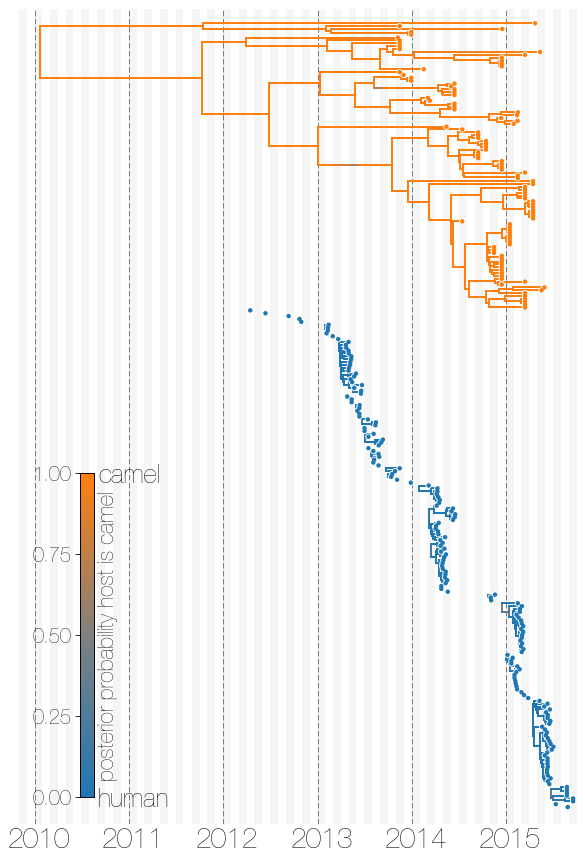
\includegraphics[width=0.65\textwidth]{figures/mers_exploded.png}
	\caption{\textbf{Evolutionary history of MERS-CoV partitioned between camels and humans.}
This is the same tree as shown in Figure \ref{mcc}, but with contiguous stretches of MERS-CoV evolutionary history split by inferred host: camels (top in orange) and humans (bottom in blue).
This visualisation highlights the ephemeral nature of MERS-CoV outbreaks in humans, compared to continuous circulation of the virus in camels.
	}
	\label{exploded}
\end{figure}

\begin{figure}[h]
\centering
	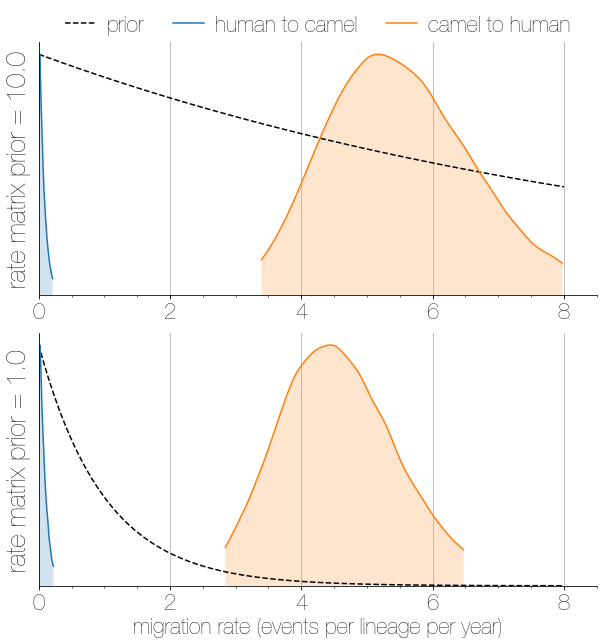
\includegraphics[width=0.65\textwidth]{figures/mers_prior.png}
	\caption{\textbf{Posterior migration rate estimates for two choices of prior.}
Negligible flow of MERS-CoV lineages from humans into camels is recovered regardless of prior choice.
Plots show the 95\% highest posterior density for the estimated migration rate from the human deme into the camel deme (blue) and \textit{vice versa} (orange).
Dotted lines indicate exponential priors specified for migration rates, with mean 1.0 (bottom) or 10.0 (top).
	}
	\label{prior}
\end{figure}


\begin{figure}[h]
\centering
	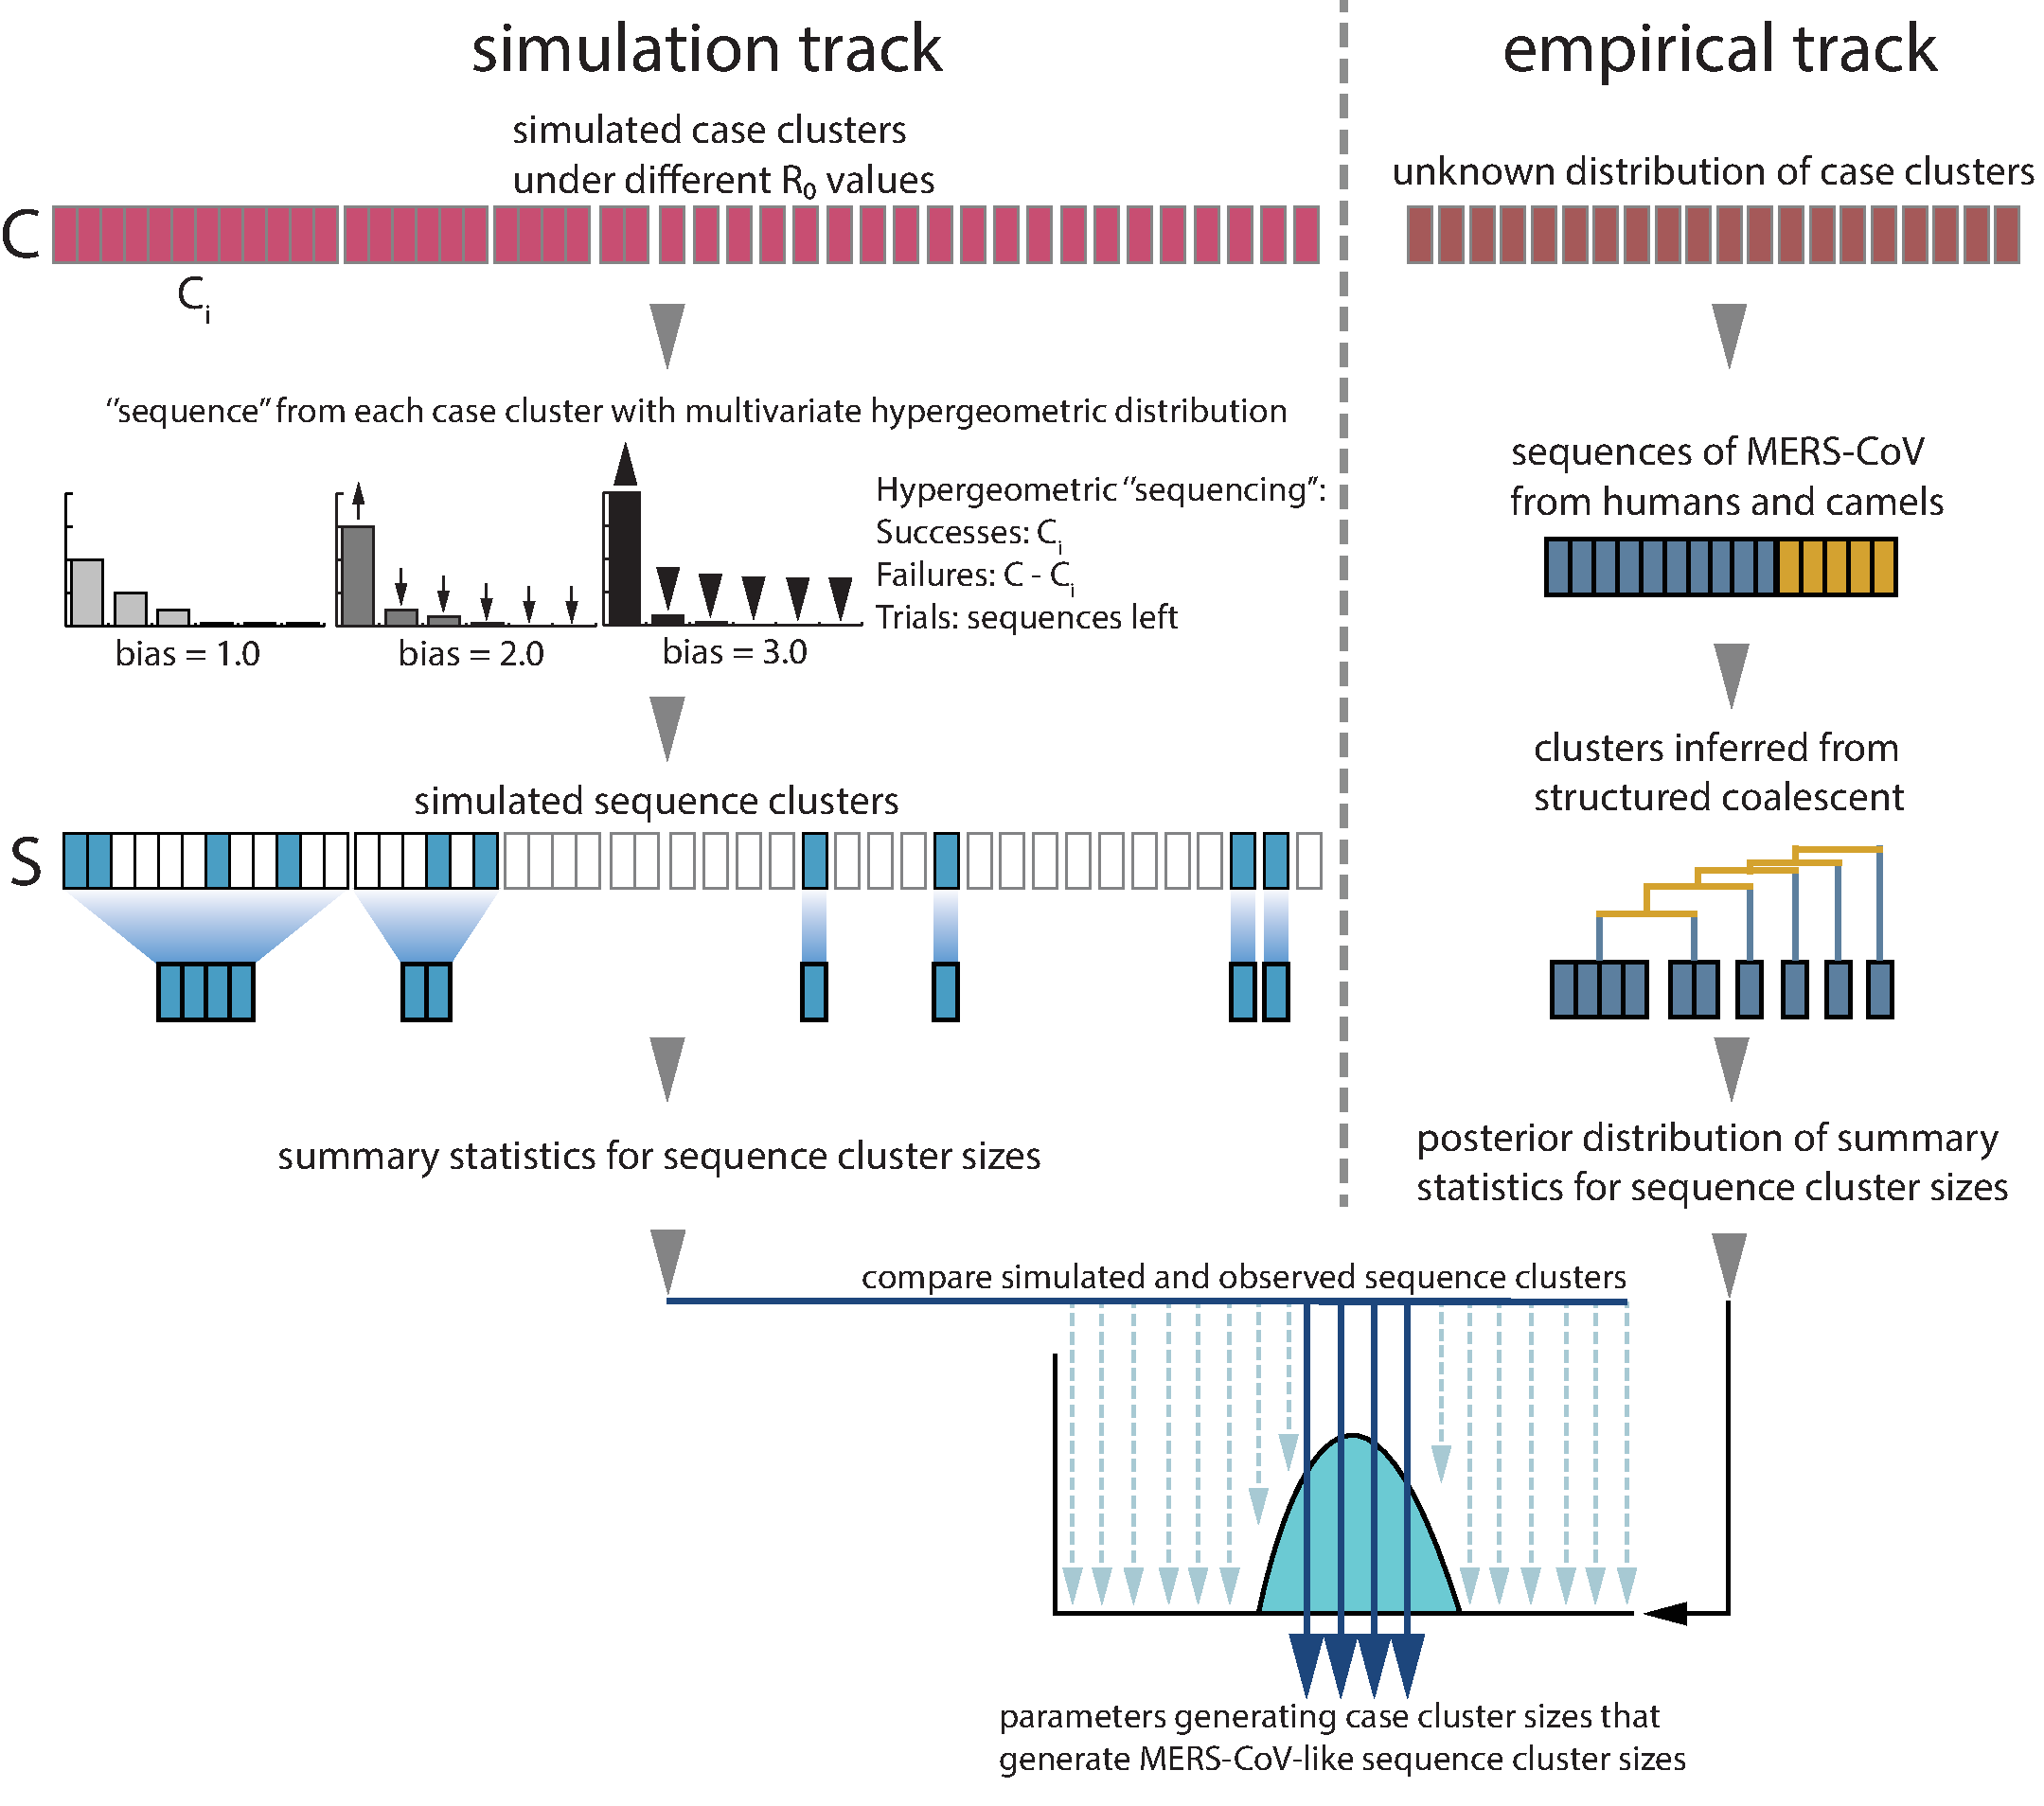
\includegraphics[width=0.75\textwidth]{figures/mers_mc_method.pdf}
	\caption{\textbf{Monte Carlo simulation schematic.}
Case clusters are simulated according to Equation \ref{clusterLikelihood} until an outbreak size of 2000 cases is reached.
We sample 174 cases from each simulation to represent sequencing of human MERS cases.
`Sequencing' is carried out by using multivariate hypergeometric sampling, representing sampling cases without replacement to be sequenced.
Sequencing simulations take place at three levels of bias: 1.0, where every case is equally likely to be sequenced, and 2.0 and 3.0, where cases from larger clusters are increasingly more likely to be sequenced.
The distribution of simulated sequence clusters is summarised by its mean, median and standard deviation.
A simulation is considered to match if the mean, median and standard deviation of its sequence cluster sizes falls within the 95\% highest posterior density interval of observed MERS-CoV sequence clusters.
$R_{0}$ values that ultimately generate data matching empirical observations, as well as associated numbers of `introductions' are retained as estimates.
These estimates are summarised in Figure \ref{mers_epi}.
	}
	\label{mc_method}
\end{figure}

\begin{figure}[h]
\centering
	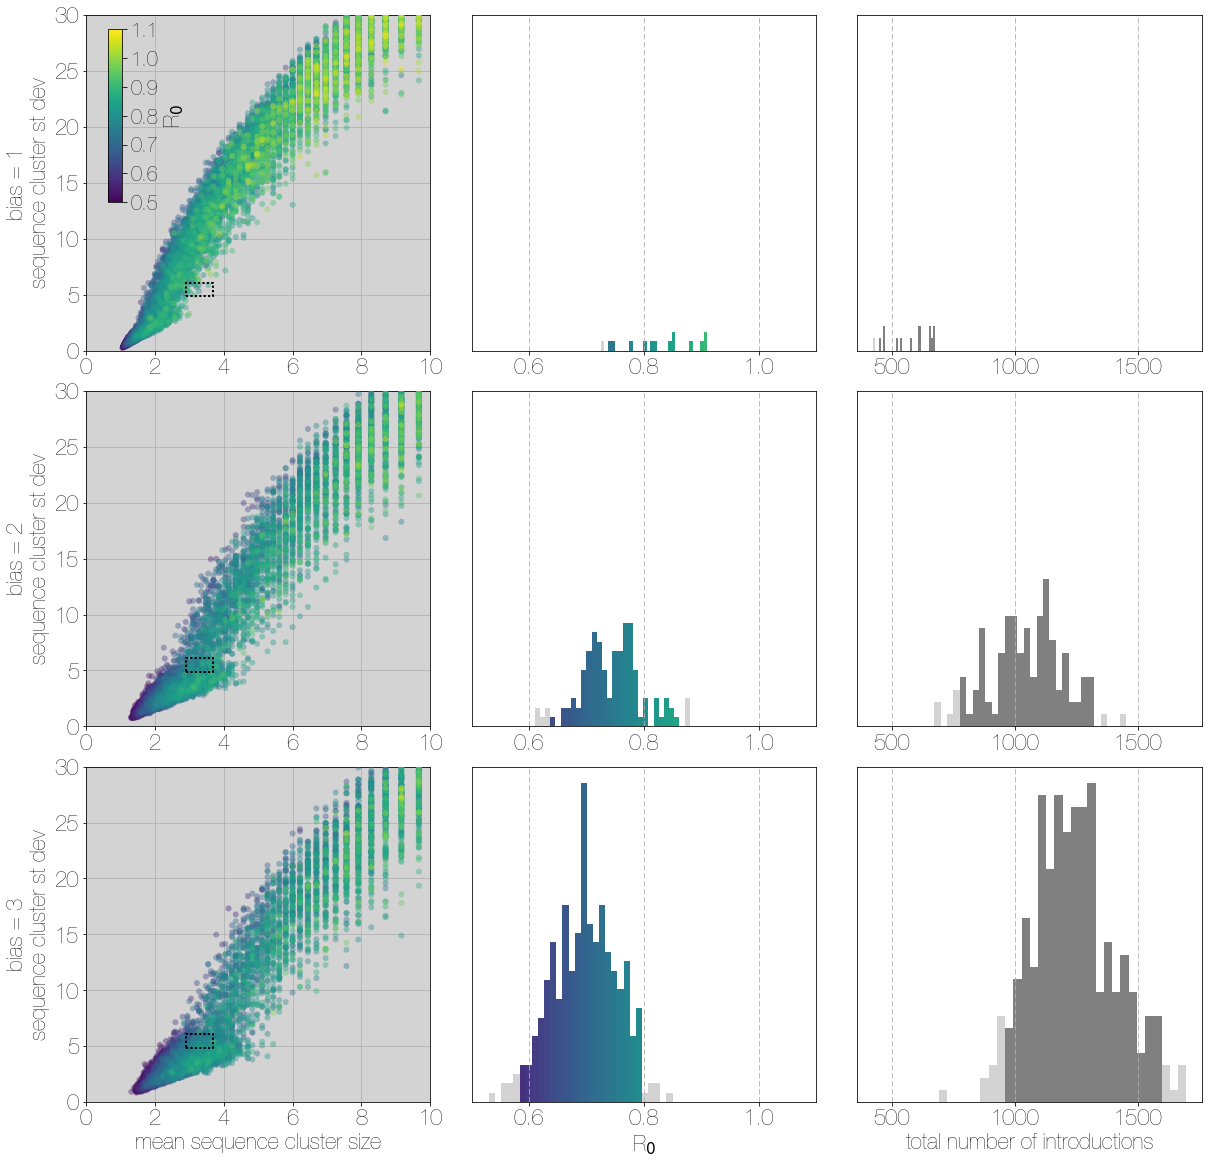
\includegraphics[width=0.65\textwidth]{figures/mers_epi_4000c.png}
	\caption{\textbf{Results of Monte Carlo simulations with vast underestimation of cases.}
The plot is identical to Figure \ref{mers_epi}, but instead of 2000 cases,
% the currently reported number of MERS-CoV cases,
simulations were run with 4000 cases.
With more unobserved cases the R$_{0}$ values matching observed MERS-CoV sequence clusters can only be smaller, with a corresponding increase in numbers of zoonotic transmissions.
However, the numbers of simulations that match MERS-CoV data go down as well.
	}
	\label{extra_cases}
\end{figure}

\begin{figure}[h]
\centering
	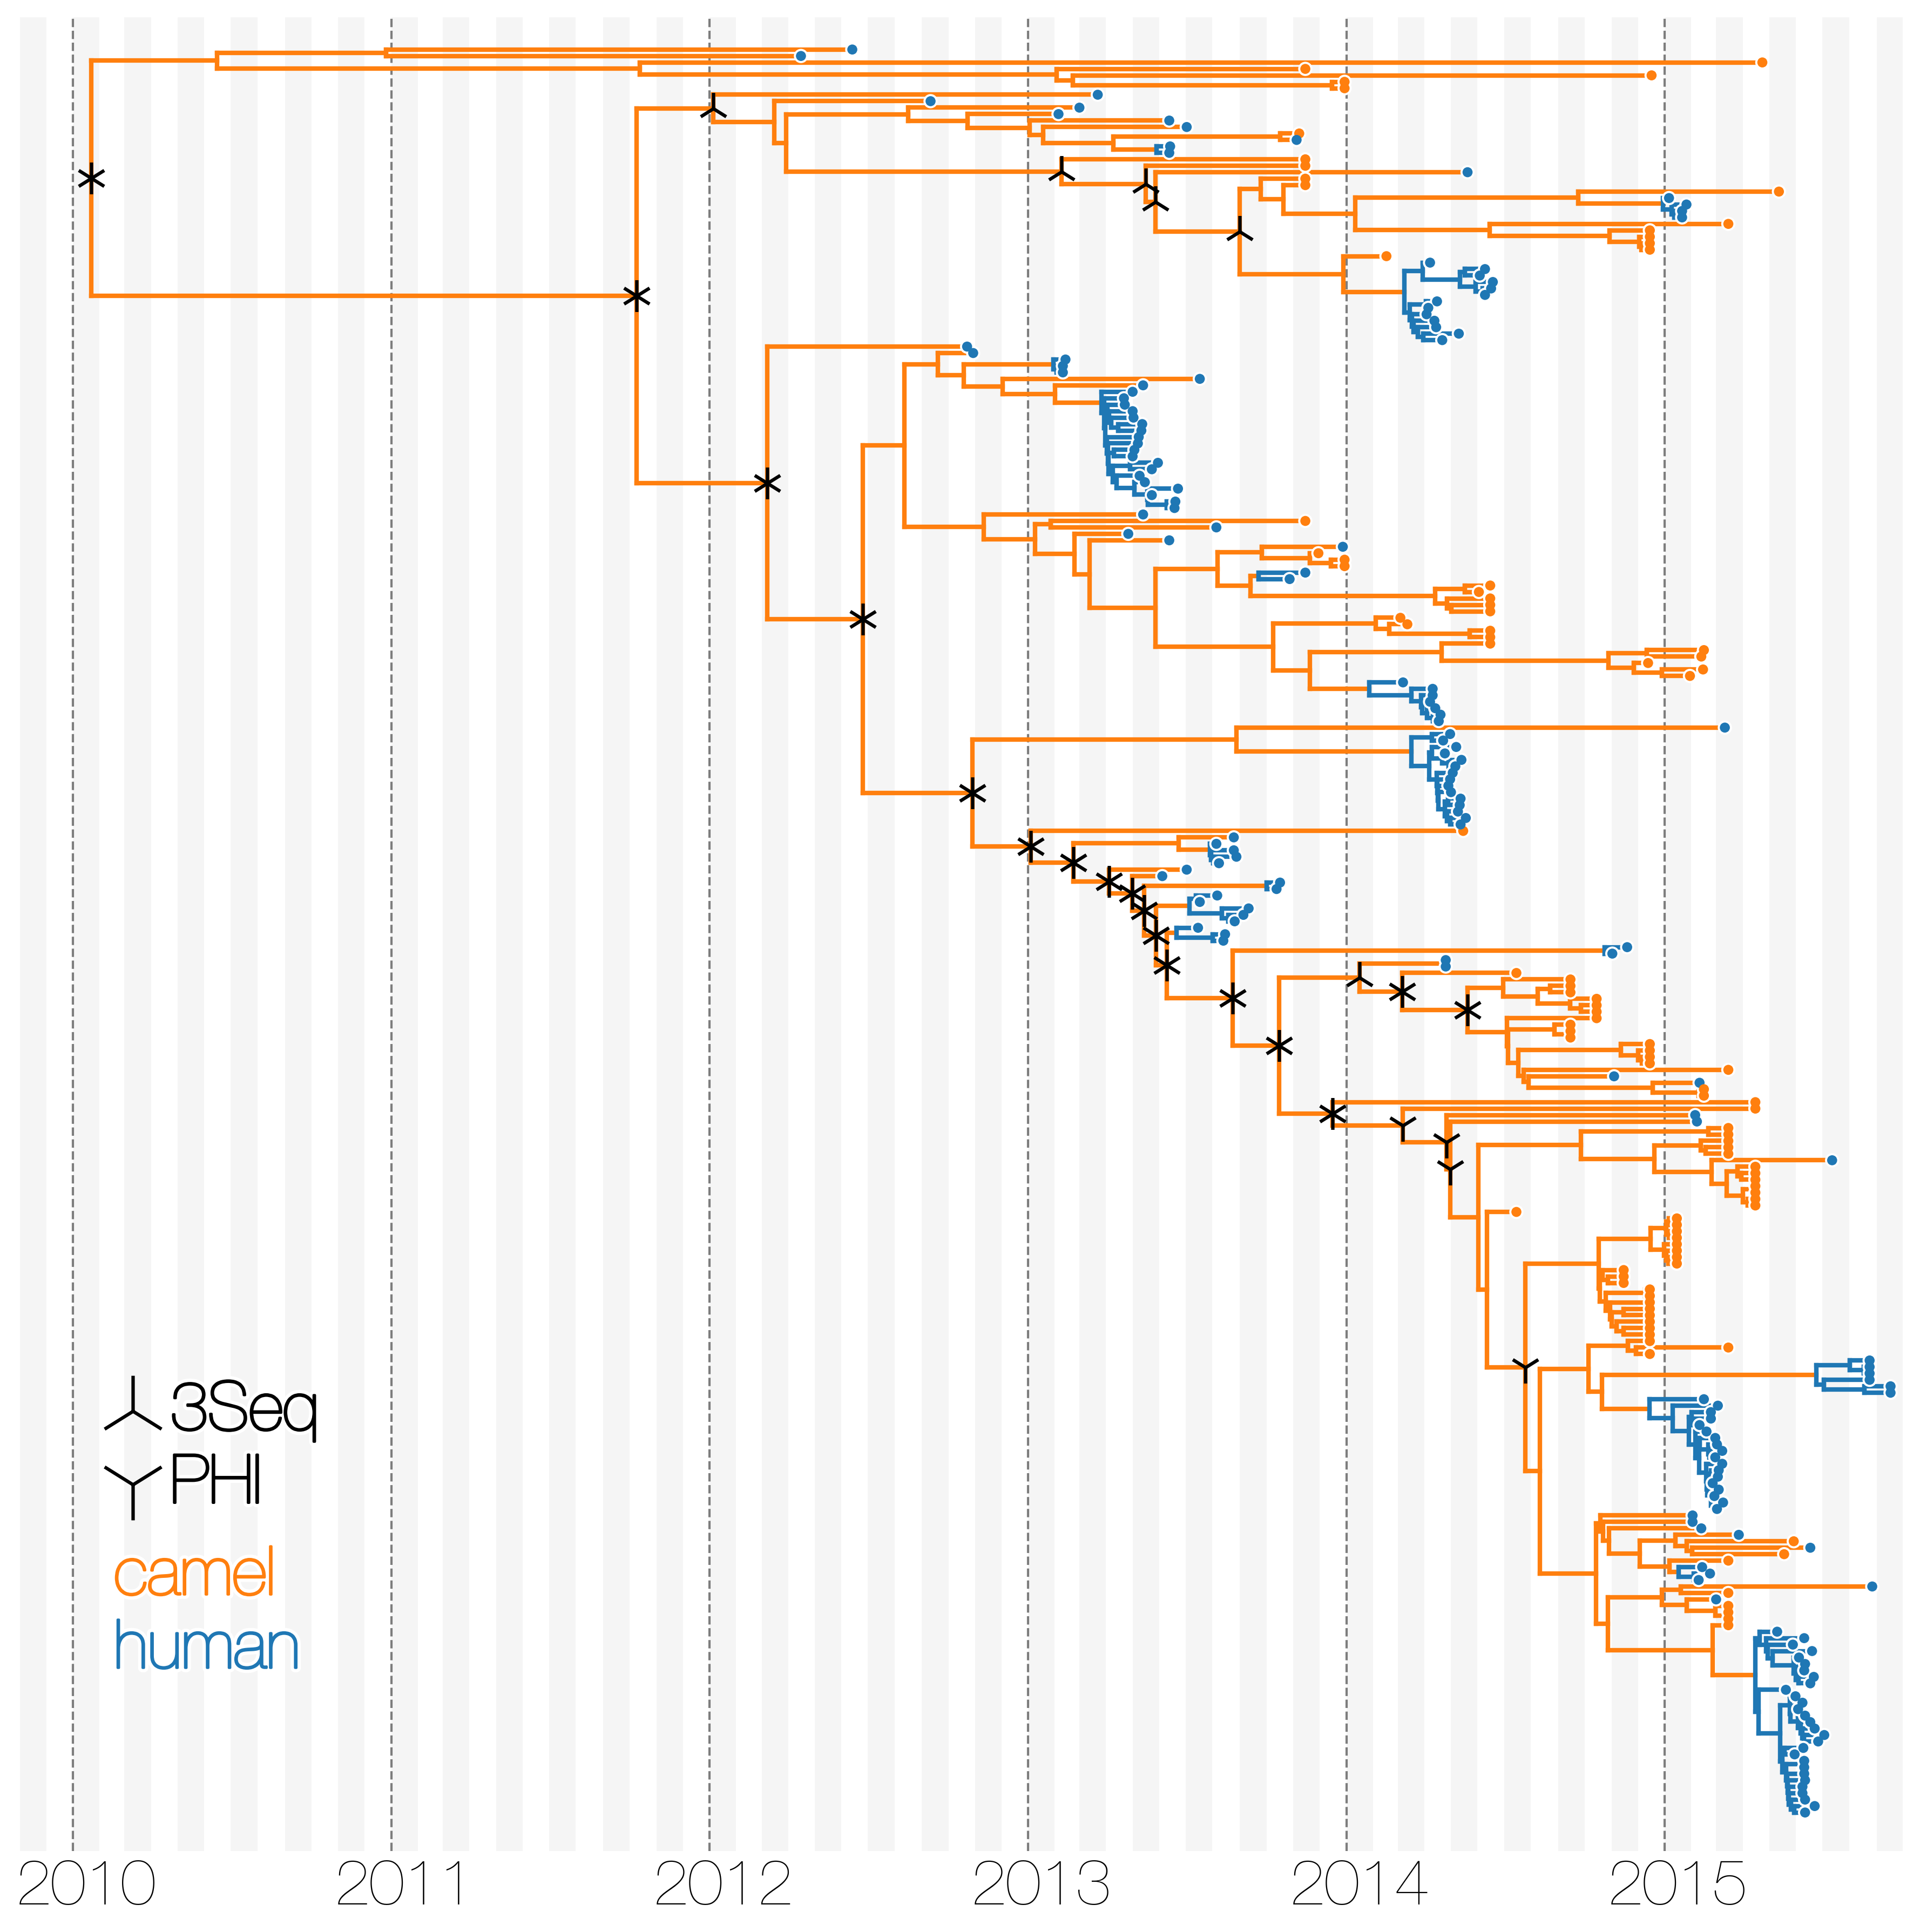
\includegraphics[width=0.65\textwidth]{figures/mers_recombination_tree.png}
	\caption{\textbf{Tests of recombination across MERS-CoV clades.}
Maximum clade credibility tree of MERS-CoV genomes annotated with results of two recombination detection tests (PHI and 3Seq) applied to descendent sequences of each clade.
Both tests identify large portions of existing sequence data as containing signals of recombination.
Note that markings do not indicate where recombinations have occurred on the tree, merely the minimum distance in sequence/time space between recombining lineages.}
	\label{recombination_tree}
\end{figure}

\begin{figure}[h]
\centering
	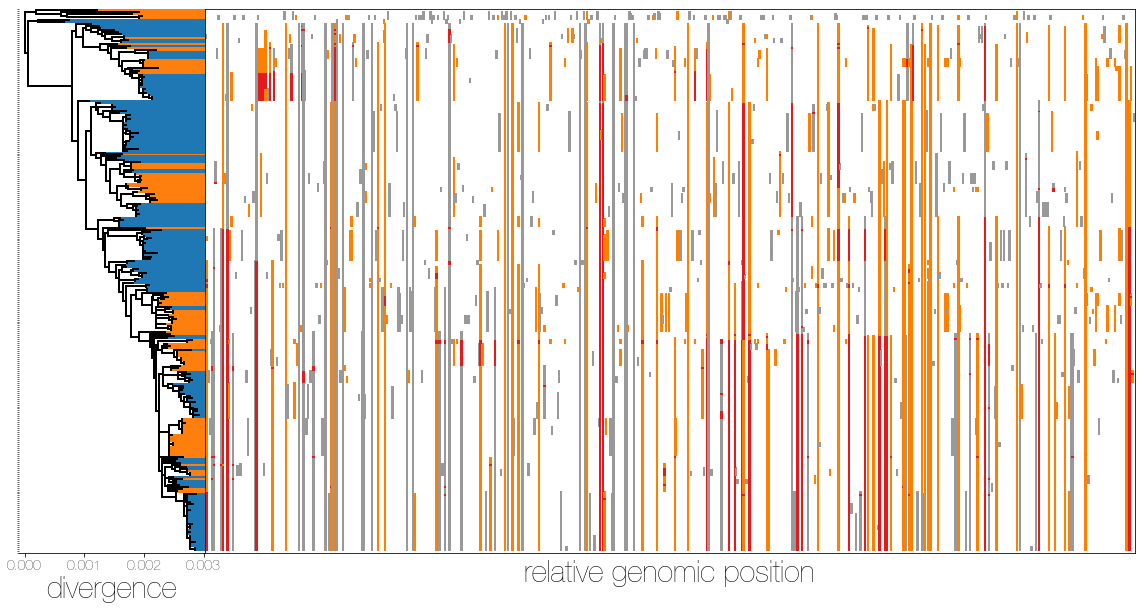
\includegraphics[width=0.75\textwidth]{figures/mers_incompatibilities.png}
	\caption{\textbf{MERS-CoV genomes exhibit high numbers of non-clonal loci.}
Ancestral state reconstruction (right) identifies a large number of sites in which mutations have occurred more than once in the tree (homoplasies, orange) or are reversions (red) from a state arising in an ancestor.
Mutations that apparently only occur once in the tree (synapomorphies) are shown in grey.
The maximum likelihood phylogeny on the left is coloured by whether sequences were sampled in humans (blue) or camels (orange).
	}
	\label{incompatibilities}
\end{figure}

\begin{figure}[h]
\centering
	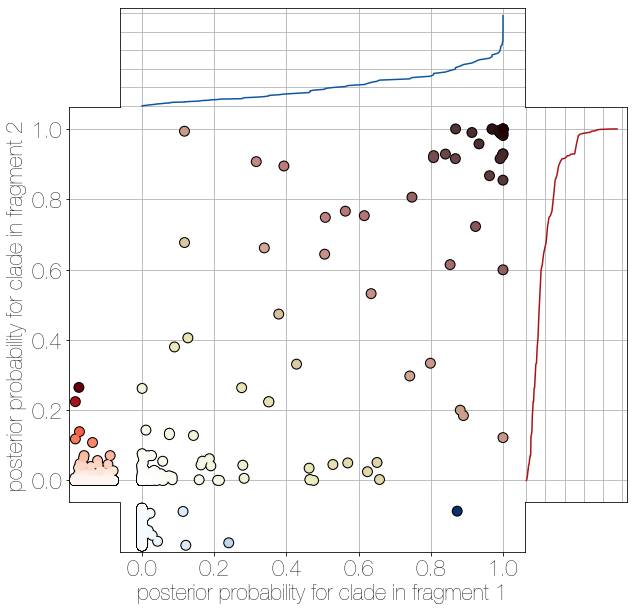
\includegraphics[width=0.65\textwidth]{figures/mers_flower.png}
	\caption{\textbf{Human clade sharing between genomic fragments 1 and 2.}
Central scatter plot shows the posterior probability of human clades shared between genomic fragments 1 and 2, in their respective trees.
Left and bottom scatter plots track the posterior probability of human clades only observed in fragment 2 (left) or fragment 1 (bottom).
The cumulative probability of human clades present in either tree are tracked by plots on the right (fragment 2) and top (fragment 1).
Most of the probability mass is concentrated within human clades that are present in trees of both genomic fragment 1 and 2 (0.9701 and 0.9474 of all human clades across posteriors, respectively).
	}
	\label{flower}
\end{figure}

\begin{figure}[h]
\centering
	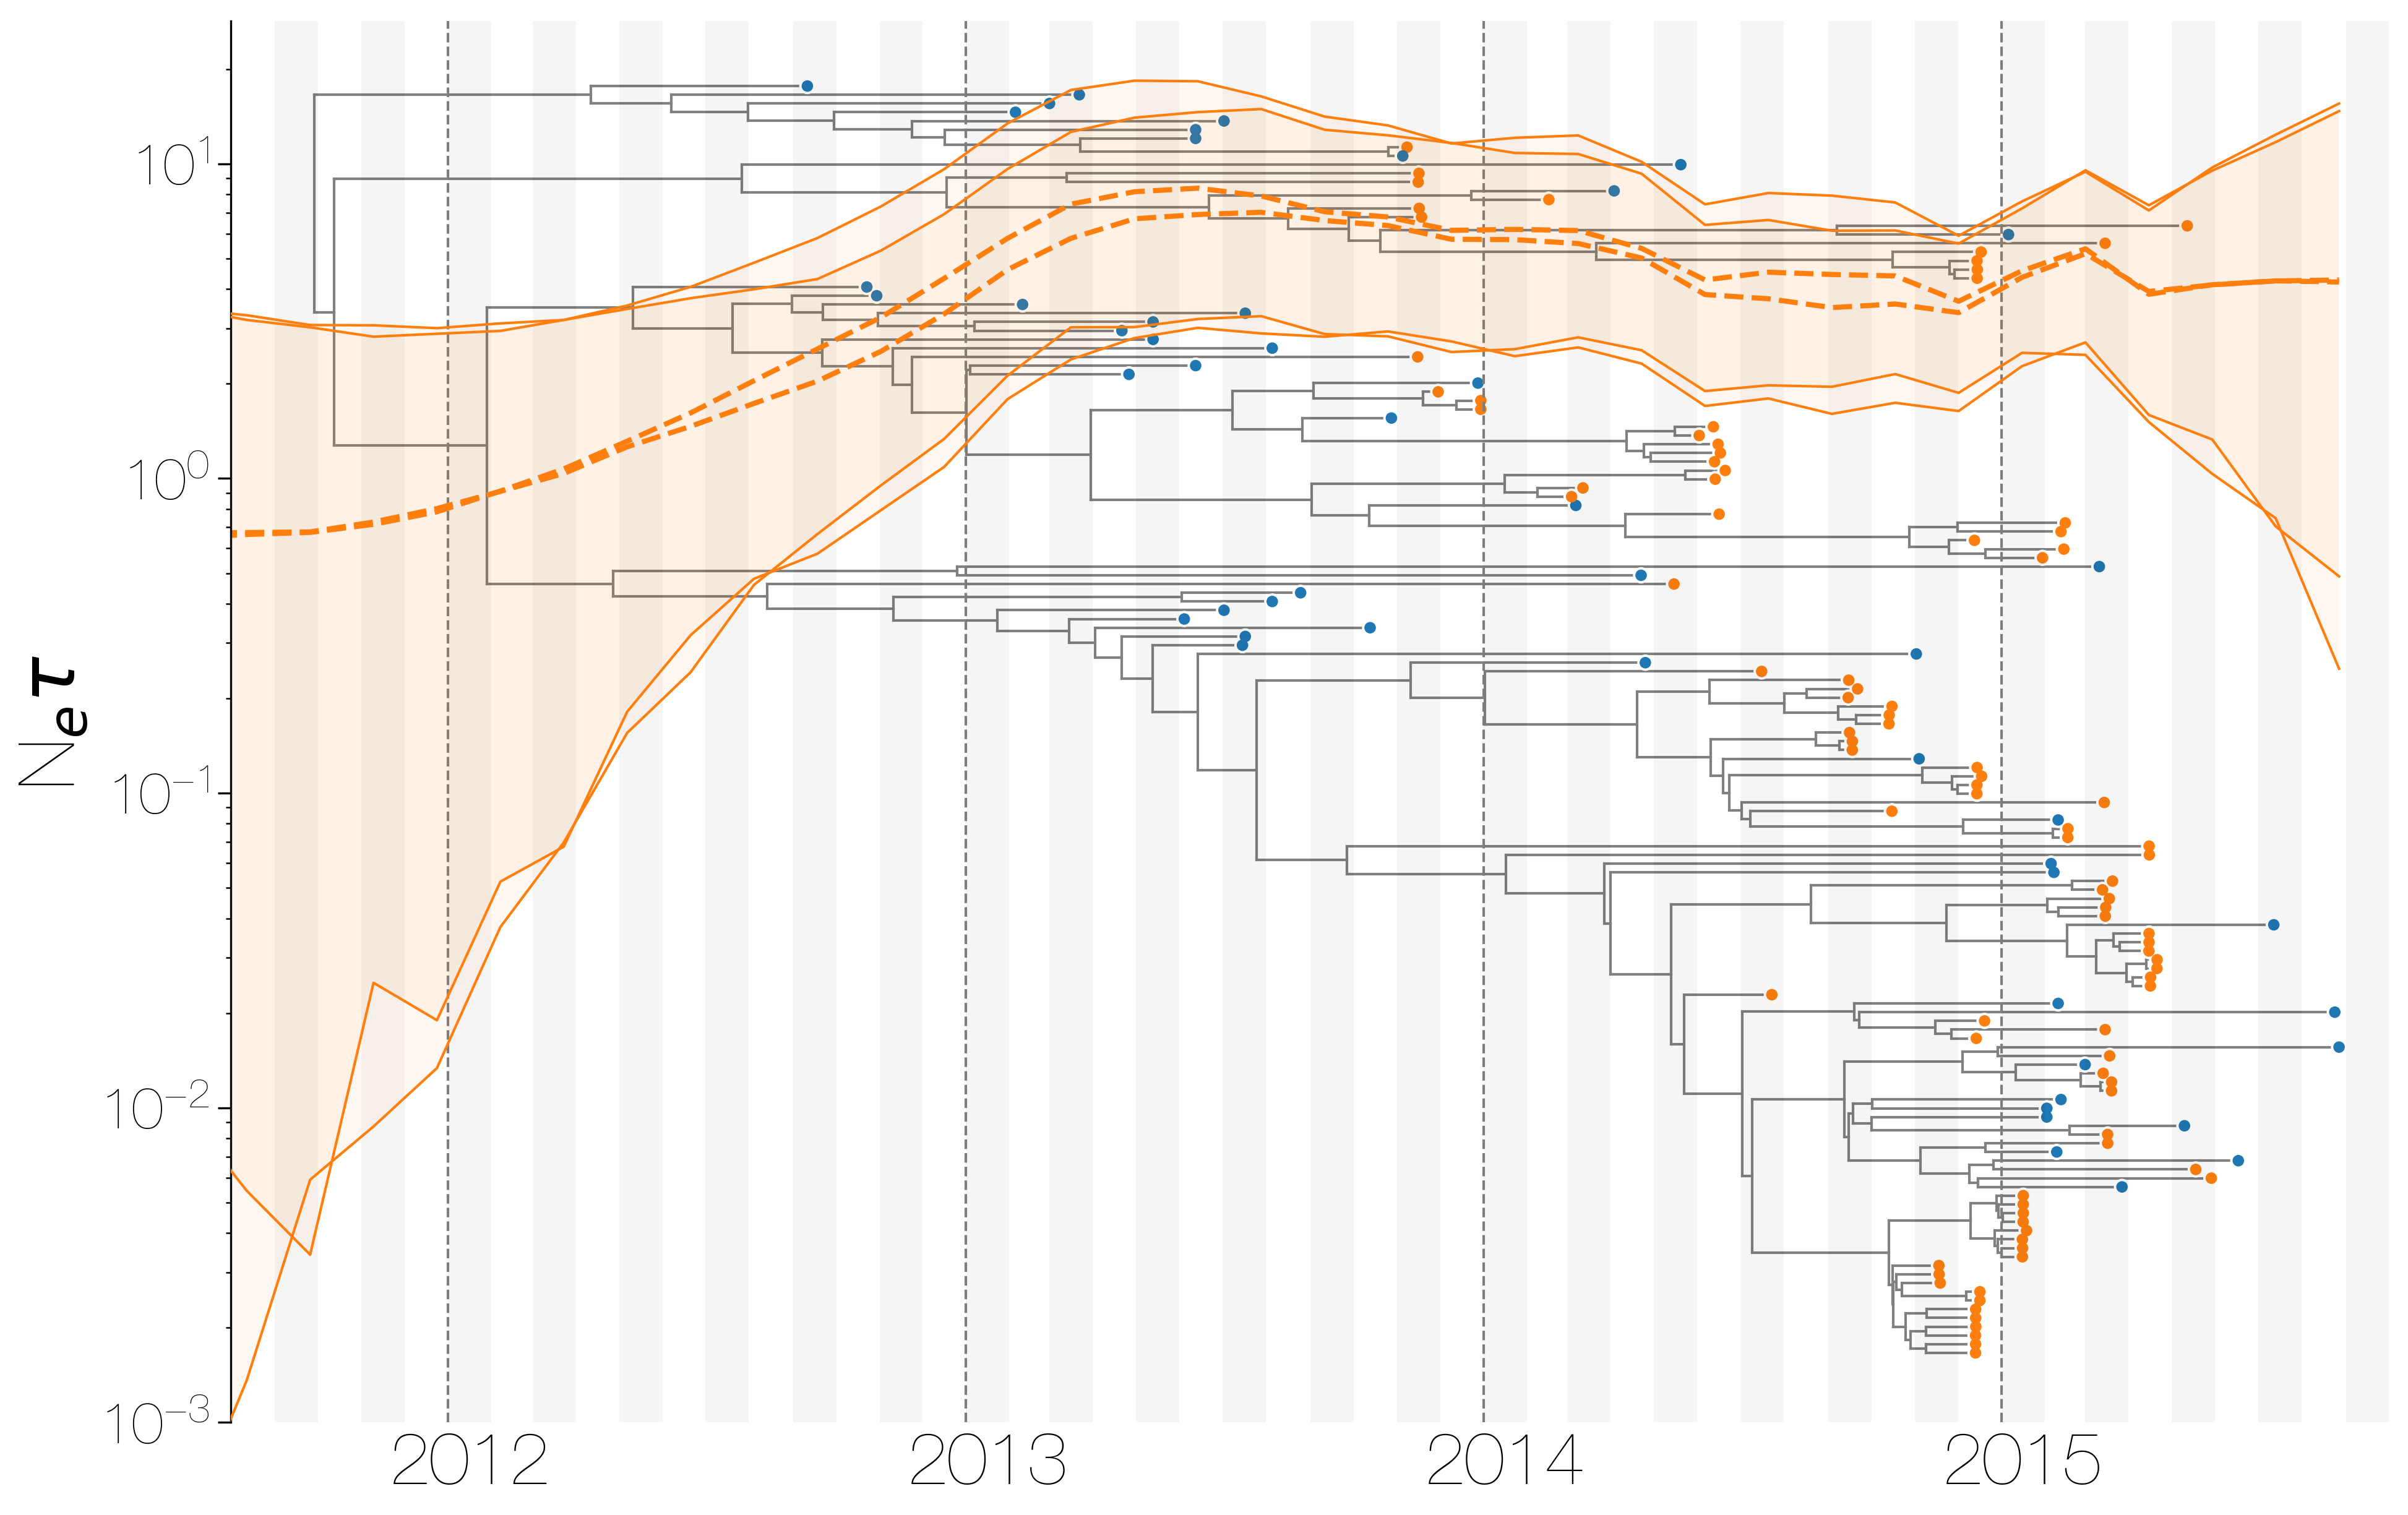
\includegraphics[width=0.65\textwidth]{figures/mers_skygrid.png}
	\caption{\textbf{Demographic history of MERS-CoV in Arabian peninsula camels.}
Demographic history of MERS-CoV in camels, as inferred via a skygrid coalescent tree prior \citep{gill_2013}.
Two skygrid reconstructions are shown, one for each of the stationary distributions reached by MCMC.
Shaded interval indicates the 95\% highest posterior density interval for the product of generation time and effective population size, $N_{e}\tau$.
Midline tracks the inferred median of $N_{e}\tau$.
Maximum clade credibility (MCC) tree from the skygrid was inferred is shown in the background, with camel sequences highlighted in orange and human sequences highlighted in blue.
	}
	\label{skygrid}
\end{figure}

\end{document}
